\documentclass{beamer}
% Use jpg graphics in figure environments and pdflatex to compile!!!
\usepackage{color,amsmath,amssymb,amsfonts,amsbsy,amsthm}
\usepackage{graphicx}
\usepackage{verbatim}
\usetheme{Berlin}
\usepackage{booktabs} 
\usepackage[english]{babel} 
\usepackage[yyyymmdd,hhmmss]{datetime}
\usepackage{subfig}
\makeatletter
\let\@@magyar@captionfix\relax
\makeatother

\newcommand{\includes}{/home/1104070/latex_include}
\newcommand{\dayonesegone}{day1_seg1_heuristic}
% Node the following tag will orient things right using dvi2pdf.
% Process with LaTeX first, then dvi2pdf.
\special{landscape}
% Fuzz -----------------------------------------------------------
\hfuzz5pt % Don't bother to report overfull boxes < 5pt
% MATH -----------------------------------------------------------

% Latex shortcuts:
\newcommand{\bfit}[1]{\textbf{\textit{#1}}}
%Decorations:
\input{\includes/taylor.tex}
\input{\includes/gensymdefs.tex}
\newcommand{\highbar}[1]{\overset{\overline{\hspace{6pt}\vspace{1pt}}}{#1}}
\newcommand{\widebar}[1]{\overset{\overline{\hspace{10pt}}}{#1}}
% Document Structure:
\newcommand{\subsubsubsection}[2]{\textbf{\arabic{section}.\arabic{subsection}.\arabic{subsubsection}.#1 #2 }}
% Sets:
\newcommand{\st}{\; : \;}
\newcommand{\set}[1]{\left\{#1\right\}}
\newcommand{\eps}{\varepsilon}
\newcommand{\demorganone}{X\setminus (A\cap B)=(X\setminus A) \cup (X\setminus B)}
\newcommand{\demorgantwo}{X\setminus (A\cup B)=(X\setminus A) \cap (X\setminus B)}
\newcommand{\simpledemorganone}{(A\cap B)'=A' \cup B'}
\newcommand{\simpledemorgantwo}{(A\cup B)'=A' \cap B'}
\newcommand{\arbunion}{\bigcup_{i\in I}A_i = \set{a: (\exists i)[i\in I \wedge a\in A_i]}}
\newcommand{\arbintersection}{\bigcap_{i\in I}A_i = \set{a: (\forall i)[i\in I \Rightarrow a\in A_i]}}
\newcommand{\intdistunion}{A\cap (B\cup C)=(A\cap B)\cup (A\cap C)}
\newcommand{\uniondistint}{A\cup(B\cap C)=(A\cup B)\cap(A\cup C)}
\newcommand{\crect}[2]{[#1,#2]\times[#1,#2]}

% Relations and Functions:
\newcommand{\dom}[1]{\text{dom}\left(#1\right)}
\newcommand{\rng}[1]{\text{rng}\left(#1\right)}
\newcommand{\To}{\longrightarrow}
% Vectors, Matrices, Norms, Dot Products

\newcommand{\scolvec}[2]{
\begin{bmatrix}
#1_1\\
\vdots\\
#1_#2 
\end{bmatrix}}

\newcommand{\coltwovec}[1]{
	\begin{bmatrix}
		#1_1\\
		#1_2 
\end{bmatrix}}

\newcommand{\scolveck}[3]{
\begin{bmatrix}
#1_1(#3)\\
\vdots\\
#1_#2(#3) 
\end{bmatrix}}

\newcommand{\coltwoveck}[2]{
	\begin{bmatrix}
		#1_1(#2)\\
		#1_2(#2) 
\end{bmatrix}}

\newcommand{\colvec}[2]{
\begin{bmatrix}
#1_1\\
#1_#2
\end{bmatrix}
}

\newcommand{\rowvec}[2]{
\begin{bmatrix}
#1_1 \ldots #1_#2
\end{bmatrix}
}

\newcommand{\rowtwovec}[2]{
	\begin{bmatrix}
		#1_1  #1_#2
	\end{bmatrix}
}

\newcommand{\colvectwo}[3]{
\begin{bmatrix}
#1_1(#3)\\
#1_#2(#3)
\end{bmatrix}
}


\newcommand{\colvecthree}[2]{
\begin{bmatrix}
#1_1^{#2}\\
#1_2^{#2}\\
#1_3^{#2} 
\end{bmatrix}}

\newcommand{\rowvecthree}[2]{
\begin{bmatrix}
#1_1^{#2}, #1_2^{#2}, #1_3^{#2} 
\end{bmatrix}}

\newcommand{\colvecsum}[3]{
\begin{bmatrix}
#1_1+#2_1\\
#1_2+#2_2\\
#1_#3+#2_#3 
\end{bmatrix}
}

\newcommand{\colvecthreesum}[2]{
#1_3+#2_3 
}

\newcommand{\colveck}[3]{
\begin{bmatrix}
#1_{#3 1}\\
#1_{#3 2}\\
#1_{#3#2} 
\end{bmatrix}
}

\newcommand{\altcolveck}[3]{
\begin{bmatrix}
#1_{1}(#3)\\
#1_{2}(#3)\\
#1_{#2}(#3) 
\end{bmatrix}}

\newcommand{\seq}[1]{\left<#1\right>}
\newcommand{\ip}[2]{\left<#1,#2\right>}
\newcommand{\dprod}[2]{#1^\top #2}  % x'x
\newcommand{\abs}[1]{\left\vert#1\right\vert}
\newcommand{\norm}[1]{\left\Vert#1\right\Vert}
\newcommand{\normsq}[1]{\dprod{#1}{#1}}
\newcommand{\essnorm}[1]{\norm{#1}_{\ess}}
\newcommand{\trace}[1]{\text{tr}\left[ #1 \right]}
\newcommand{\varlist}[2]{#1=1,\ldots,#2}
\newcommand{\genmat}[1]{\left[ #1 \right]}
\newcommand{\mat}[3]{
\begin{bmatrix}
#1_{11}&\cdots&#1_{1#3}\\
\vdots&\ddots&\vdots\\
#1_{#2 1}&\cdots & #1_{#2#3} 
\end{bmatrix}}
%\newcommand{\trans}{^{\textsc{\begin{tiny}T\end{tiny}}}}
\newcommand{\trans}{^\top}
\newcommand{\B}{
\begin{bmatrix} 
0\\
K
\end{bmatrix}
}
\newcommand{\C}{
\begin{bmatrix} 
b_o & b_1 & \cdots & b_{m-1}
\end{bmatrix}
}
\newcommand{\skewsymmat}[4]{
\begin{bmatrix}
 0 & -#1_{#4} & #1_{#3}\\
 #1_{#4}& 0 & -#1_{#2}\\
-#1_{#3} & #1_{#2} & 0
\end{bmatrix}
}
\newcommand{\skewsymmatone}[4]{
\begin{bmatrix}
 1 & -#1_{#4} & #1_{#3}\\
 #1_{#4}& 1 & -#1_{#2}\\
-#1_{#3} & #1_{#2} & 1
\end{bmatrix}
}
% State Space Notation:
\newcommand{\qloss}{\tilde{x}^\top\tilde{x}} %\top = top TRUE symbol in logic used for transpose.
\newcommand{\Gint}{\int_{t_0}^{t}\Phi(t,\tau)G(\tau)w(\tau)d\tau}
\newcommand{\Lint}{\int_{t_0}^{t}\Phi(t,\tau)L(\tau)u(\tau)d\tau}
\newcommand{\Xhat}{\hat{X}_i(t)}
\newcommand{\Xo}{X_{0i}(t)}
\newcommand{\xdot}{\colvec{\dot{x}}{n}}
\newcommand{\state}{\scolvec{x}{n}}
\newcommand{\statek}{\scolveck{x}{n}{k}}
\newcommand{\procnoisek}{\scolveck{w}{n}{k}}
\newcommand{\altstatek}{\altcolveck{x}{n}{k}}
\newcommand{\sxdot}{\scolvec{\dot{x}}{n}}
\newcommand{\sstate}{\scolvec{x}{n}}
\newcommand{\expstm}{\exp\left[A(t-t_0)\right]}
\newcommand{\expstmalt}{\exp\left[F(t-t_0)\right]}
% Kalman Specific Notation:
\input{\includes/kfspecific.tex}
% Statistical Notation:
\newcommand{\gvpdf}{\frac{1}{\sqrt{(2\pi)^n \det(C)}}
  \exp\left[ -\frac{1}{2}(x-\mu)\trans C^{-1} (x-\mu) \right]}
\newcommand{\variance}[1]{\text{Var}(#1)}
\newcommand{\sigsq}[1]{\sigma^2_{#1}}
\newcommand{\cov}[2]{\text{Cov}(#1,#2)}
\newcommand{\covdef}[2]{\cov{#1}{#2}:=\expect{(#1-\mu{#1})(#2-\mu{#2})}}
\newcommand{\corrdef}[2]{\rho_{#1#2}:=\dfrac{\cov{#1}{#2}}{\sigma_{#1}\sigma_{#2}}}
\newcommand{\std}[1]{\sqrt{\variance{#1}}}
\newcommand{\expect}[1]{\text{E}\left[#1\right]}
\newcommand{\shortexp}[1]{\text{E}#1}
\newcommand{\msconv}{\xrightarrow{\text{m.s.}}}
\newcommand{\samplemean}[1]{\bar{#1}}
\newcommand{\samplemeandef}[1]{\samplemean{#1}:=\dfrac{1}{N}\sum_{i=1}^{N} #1_{i}}
\newcommand{\samplevar}[1]{s^2_{#1}}
\newcommand{\samplevardef}[1]{\samplevar{#1}:=\dfrac{1}{N-1}\sum_{i=1}^{N} (#1_{i}-\samplemean{#1})^2}
\newcommand{\samplecov}[2]{s^2_{#1#2}}
\newcommand{\samplecovdef}[2]{s^2_{#1#2}:=\dfrac{1}{N-1}\sum_{i=1}^{N}(#1-\samplemean{#1})(#2-\samplemean{#2})}
\newcommand{\samplecorrdef}[2]{r_{#1#2}:=\dfrac{\samplecov{#1}{#2}}{s_{#1}s_{#2}}}
% Various integrals:
\newcommand{\minfint}[1]{\underbrace{\int_{-\infty}^{+\infty}\cdots}}
\newcommand{\rsintfull}[4]{\int_{#1}^{#2}#3(t)d#4(t)}
\newcommand{\rsint}[2]{\rsintfull{a}{b}{#1}{#2}}
\newcommand{\drsint}[2]{\iint\limits_{\crect{a}{b}}#1(s)#1(t)d_{s}d_{t}#2(s,t)}
\newcommand{\rint}[1]{\int_{a}^{b}#1dt}
\newcommand{\infint}{\int\limits_{-\infty}^{\infty}}
\newcommand{\limint}{\lim_{T\rightarrow \infty}\frac{1}{T}\int_0^T}
\newcommand{\halfint}{\int\limits_0^{\infty}}
\newcommand{\halfintplus}{\int\limits_{0^+}^{\infty}}
% Derivatives:
\newcommand{\deriv}[2]{\dfrac{d#1}{d#2}}
\newcommand{\secondderiv}[2]{\dfrac{d^2#1}{d#2^2}}
\newcommand{\pderiv}[2]{\dfrac{\partial#1}{\partial#2}}
\newcommand{\ppderivop}[1]{\dfrac{\partial^2}{\partial#1^2}}
%\newcommand{\pderiv}[1]{\left[\partial / \partial #1\right]}
\newcommand{\grad}[2]{\dfrac{\partial #1}{\partial #2}}
% Differential and Difference equations:
\newcommand{\diffeq}{\sum_{i=0}^{n}a_i\frac{d^iy}{dt^i} = \sum_{i=0}^{m}b_i\frac{d^iu}{dt^i}}
\newcommand{\armaeq}{\sum_{i=0}^na_{n-i}y(k+n-i) = \sum_{i=0}^mb_{m-i}u(k+m-i)}
\newcommand{\armaeqfull}{a_ny(n+k)+\cdots+a_0y(k)=b_mu(k+m)+\cdots+b_0y(k)}
\newcommand{\companion}{
\begin{bmatrix}
0 & 1 & 0 & \cdots & 0 & 0\\
0 & 0 & 1 & \cdots & 0 & 0\\
\vdots &  &  &  &  & \vdots\\
0 & 0 & 0 & \cdots & 0 & 0\\
-a_0 & -a_1 & -a_2 & \cdots & -a_{n-2} & -a_{n-1}
\emd{bmatrix}
}
\newcommand{\taylor}[3]{#1(#2)=#1(#3)+\dot{#1}(#3)(#2-#3)+\frac{1}{2!}\ddot{#1}(#3)(#2-#3)^2+\cdots}
\newcommand{\gentaylorsingle}[3]{#1(#2)=#1(#3)+\dfrac{d#1}{d#2}(#3)(#2-#3)+\dfrac{1}{2!}\dfrac{d^2#1}{d#2^2}(#3)(#2-#3)^2+\cdots}
\newcommand{\gentaylordouble}[5]{#1(#2,#3)
&=#1(#4,#5)+#1_{#2}(#4,#5)(#2-#4)+#1_{#3}(#4,#5)(#3-#5)\\
&+\;\;\;\dfrac{1}{2!}(#1_{#2#2}(#4,#5)(#2-#4)^2\\
&+\;\;\;\;\;\;#1_{#2#3}(#4,#5)(#2-#4)(#3-#5)\\
&+\;\;\;\;\;\;#1_{#3#3}(#4,#5)(#3-#5)^2)+\cdots}
% Harmonic Oscillator Equations
\newcommand{\harmoscdiffeqhom}{m\ddot{x}+c\dot{x}+kx=0}
\newcommand{\harmoscdiffeqnonhom}{m\ddot{x}+c\dot{x}+kx=w(t)}
\newcommand{\productrule}{D(f\cdot g)=[Df]\cdot g+f\cdot [Dg]}
\newcommand{\chainrule}{D(f\circ g) = [Df]\circ g \cdot [Dg]}
\newcommand{\multichainrule}{D(f\circ g\circ h) = ([Df]\circ g \circ h) \cdot ([Dg] \circ h) \cdot [Dh]}
\newcommand{\compdist}{(f\cdot g)\circ h=(f\circ h) \cdot (g\circ h)}
\newcommand{\zetaf}[1]{\exp\left[\frac{1}{#1^2-1}\right]}
\newcommand{\laplace}{F(s)=\mathcal{L}[f(t)]=\int_{0^+}^{\infty}f(\tau)\exp(-s\tau)d\tau}
\newcommand{\ithrow}[2]{#1_{(#2)}}
\newcommand{\jthcol}[2]{#1^{(#2)}}
\newcommand{\ijthelem}[1]{\left[ #1 \right]_{(i,j)}}
% INS/GPS specific:
\input{\includes/insgpsdefs.tex}
% Navigation Quantities:
\input{\includes/naveqdefs.tex}
% Error Dynamics Equations:
\input{\includes/errdyneqdefs.tex}
% rate integrals:
\newcommand{\eratevec}{\rotvec{I}{E}}
\newcommand{\rotvec}[2]{\omega_{#1#2}}
\newcommand{\rotmat}[2]{\Omega_{#1#2}}
\newcommand{\erate}{\Omega_e}
\newcommand{\eradius}{R_e}
\newcommand{\erateval}{\erate=7.2921151467\times 10^{-5} \text{ rad/sec}}
\newcommand{\eradiusval}{\eradius=6,378,137 \text{ meters}}
\newcommand{\eratex}{\Omega_x}
\newcommand{\eratexeq}{\eratex&=\erate\cos\lat\sin\alpha}
\newcommand{\eratey}{\Omega_y}
\newcommand{\erateyeq}{\eratey&=\erate\cos\lat\cos\alpha}
\newcommand{\eratez}{\Omega_z}
\newcommand{\eratezeq}{\eratez&=\erate\sin\lat}
\newcommand{\avgearth}{\highbar{\Omega}_i}
\newcommand{\avgeartheq}{\avgearth = \intdeltaT \Omega_i(t) dt,\forxyz}
% relative rates or transport rates:
\newcommand{\trate}{\rotvec{E}{L}}
\newcommand{\avgrelvec}{\highbar{\rho}}
\newcommand{\avgrel}{\highbar{\rho}_i}
\newcommand{\avgreleq}{\avgrel=\intdeltaT \rho_i dt,\forxyz}
\newcommand{\avgrelx}{\highbar{\rho}_x}
\newcommand{\avgrelxeq}{\avgrelx&=-\dfrac{\highbar{V}_y}{R}}
\newcommand{\avgrely}{\highbar{\rho}_y}
\newcommand{\avgrelyeq}{\avgrely&=\dfrac{\highbar{V}_x}{R}}
\newcommand{\avgrelz}{\highbar{\rho}_z}
\newcommand{\avgrelxspheroideq}{\avgrelx&=
-\dfrac{\highbar{V}_y}{R}(1-\dfrac{h}{R})}
\newcommand{\avgrelyspheroideq}{\avgrely&=\dfrac{\highbar{V}_x}{R}}
\newcommand{\avgspatial}{\highbar{\omega}_i}
\newcommand{\avgspatialeq}{\avgspatial = \avgearth + \avgrel,\forxyz}
\newcommand{\avgCoriolis}{\highbar{\omega}_{ci}}
\newcommand{\avgCorioliseq}{\avgCoriolis=\avgearth + \avgspatial}
\newcommand{\Schulerfreq}{\omega_s}
\newcommand{\Schulerfreqeq}{\Schulerfreq = \sqrt{\frac{g}{R}}}
\newcommand{\localgeq}{g=\dfrac{A^2}{R^2}g_0}
% body to nav transforms:
\newcommand{\dcm}[2]{C_{#1}^{#2}}
\newcommand{\compdcm}[2]{\widehat{C}_{#1}^{#2}}
\newcommand{\bodytoll}{C_B^L}
\newcommand{\lltoearth}{C_L^E}
\newcommand{\earthtoll}{C_E^L}
\newcommand{\bodytonav}[1]{C_B^L(#1)}
\newcommand{\Ctminuseq}{\bodytonav{t^{-}}=\Ctzero \bodytonav{0}}
\newcommand{\Ctzero}{C_{t0}}
\newcommand{\Ctzeroeq}{
C_{t0}=\bodytonav{t^{-}}\bodytonav{0}\trans=
\skewsymmatone{p}{x}{y}{z} + 2^{\text{nd}}\text{ order terms} }
\newcommand{\Ctzerocomm}[2]{\dfrac{1}{2}\left[\Ctzero(#1,#2)-\Ctzero(#2,#1)\right]}
\newcommand{\peq}[3]{p_{#1}&=\dfrac{\theta_{#1} }
{\theta}\sin\theta=\Ctzerocomm{#2}{#3}}
\newcommand{\avgbodytoll}{\highbar{C}_B^L}
\newcommand{\avgbodytolleq}{\avgbodytoll=\intdeltaT \bodytoll dt}
\newcommand{\croll}{\cos\phi}
\newcommand{\sroll}{\sin\phi}
\newcommand{\cpitch}{\cos\theta}
\newcommand{\spitch}{\sin\theta}
\newcommand{\cyaw}{\cos\psi}
\newcommand{\syaw}{\sin\psi}
\newcommand{\bodytolleq}{\bodytoll&=
\cpitch\syaw & \syaw\spitch\sroll+\cyaw\croll & \syaw\spitch\croll
- \cyaw\sroll\\
\cpitch\cyaw & \cyaw\spitch\sroll-\syaw\croll &
\cyaw\spitch\croll+\syaw\sroll\\
\spitch & -\cpitch\sroll & -\cpitch\croll
}
% Integrals of velocity (average velocity):
\newcommand{\avgvelvec}{\highbar{V}}
\newcommand{\avgvel}{\highbar{V}_i}
\newcommand{\avgveleq}{\avgvel=\intdeltaT V_i dt, \forxyz}
\newcommand{\sensedaccel}{\highbar{A}_{Bi}}
\newcommand{\sensedacceleq}{\sensedaccel = \intdeltaT A_{Bi} dt, \forXYZ}
\newcommand{\sensedrate}{\highbar{\omega}_{Bi}}
\newcommand{\sensedrateeq}{\sensedrate = \intdeltaT \omega_{Bi} dt, \forXYZ}
\newcommand{\sensedaccellev}{\highbar{A}_{L}}
\newcommand{\sensedaccelleveq}{\sensedaccellev = \intdeltaT \bodytoll A_{B} dt}
\newcommand{\avgbodyaccel}{A_{aBi}}
\newcommand{\avgbodyacceleq}{\avgbodyaccel=\frac{\sensedaccel}{\Delta T}, \forXYZ}
\newcommand{\avgbodyrate}{\omega_{aBi}}
\newcommand{\avgbodyrateeq}{\avgbodyrate=\frac{\sensedrate}{\Delta T}, \forXYZ}
\newcommand{\psix}{\psi_x}
\newcommand{\psixeq}{\psix &= \phi_x + \frac{\Delta R_y}{R}}
\newcommand{\psiy}{\psi_y}
\newcommand{\psiyeq}{\psiy &= \phi_y - \frac{\Delta R_x}{R}}
% Position Derivatives:
\newcommand{\posderivx}{\delta R_x}
\newcommand{\posderivxeq}{\posderivx &= \Delta V_x \Delta T+\highbar{V}_y\psi_z-\highbar{V}_z\phi_y-\avgrely\Delta R_z}
\newcommand{\stmposerrxeq}{\poserr_x(k+1)=\poserr_x(k)+
0 & 0 & \avgrely & \Delta T & 0 & 0 & 0 & -\highbar{V}_z &
\highbar{V}_y & 0\; \cdots
\state}
\newcommand{\posderivy}{\delta R_y}
\newcommand{\posderivyeq}{\posderivy &= \Delta V_y \Delta T+\highbar{V}_z\phi_x-\highbar{V}_x\psi_z+\avgrelx\Delta R_z}
\newcommand{\posderivz}{\delta R_z}
\newcommand{\posderivzeq}{\posderivz &= \Delta V_z \Delta T+\highbar{V}_x\phi_y-\highbar{V}_y\phi_x+\avgrely\Delta R_x-\avgrelx\Delta R_y}
\newcommand{\posderiv}{\delta R}
\newcommand{\posderiveq}{\posderiv = \Delta V \Delta T + \highbar{V}\times \psistar - \avgrelvec \times \Delta R}
% Attitude Derivatives:
\newcommand{\attderivx}{\delta \phi_x}
\newcommand{\attderivxeq}{\attderivx &= \highbar{\omega}_z \psi_y -\highbar{\omega}_y\psi_z-\frac{\delta R_y}{R}+\highbar{\epsilon}_x}
\newcommand{\attderivy}{\delta \phi_y}
\newcommand{\attderivyeq}{\attderivy &= \highbar{\omega}_x \psi_z -\highbar{\omega}_z\psi_x+\frac{\delta R_x}{R}+\highbar{\epsilon}_y}
\newcommand{\attderivz}{\delta \psi_z}
\newcommand{\attderivzeq}{\attderivz &= \highbar{\omega}_y \psi_x -\highbar{\omega}_x\psi_y+\highbar{\epsilon}_z}
% Psi and Psi*
\newcommand{\psistar}{\psi^*}
\newcommand{\psistareq}{\psistar =
\phi_x\\
\phi_y\\
\psi_z
}
\newcommand{\dpsistar}{\delta\psi^*}
\newcommand{\dpsistareq}{\dpsistar =
\delta\phi_x\\
\delta\phi_y\\
\delta\psi_z
}
\newcommand{\psieq}{\psi =
\psi_x\\
\psi_y\\
=
\phi_x + \vspace{5 pt}\dfrac{\Delta R_y}{R}\\
\phi_y - \dfrac{\Delta R_x}{R}
}
\newcommand{\psidoteq}{\dot{\psi}=-\omega\times\psi+\epsilon}
\newcommand{\angposerr}{\delta \theta}
\newcommand{\angposerreq}{\angposerr=
-\dfrac{\Delta R_y}{R}\vspace{5 pt}\\
\;\;\dfrac{\Delta R_x}{R}\;\vspace{5 pt}\\
0}
\newcommand{\xop}[1]{\left[\; #1\times \; \right]}
\newcommand{\xopdef}[1]{
\begin{bmatrix}
0 & #1_z & -#1_y\\
-#1_z & 0 & #1_x\\
#1_y & -#1_x & 0
\end{bmatrix}
}
\newcommand{\vxomegax}{\xop{V}\xop{\Omega}}
\newcommand{\vxomegaxeq}{\vxomegax=\xopdef{V}\xopdef{\Omega}}
\newcommand{\T}{T}
\newcommand{\Teq}{\T=\frac{1}{\Delta T}\left[ \dpsistar + \highbar{\omega}_c\times \psistar \right]}
\newcommand{\altTeq}{\T=\frac{1}{\Delta T}\left[\: \highbar{\Omega}\times \psistar + \highbar{\epsilon}\: \right]}
\newcommand{\dV}{\delta V}
\newcommand{\dVeq}{\dV=\Delta V\times \highbar{\omega}_c + \T\times \highbar{V} }
\newcommand{\altdVeq}{\dV=\Delta V\times \highbar{\omega}_c + \T\times \highbar{V} }
\newcommand{\Corratecrossop}{\xop{\highbar{\omega}_c}}
\newcommand{\Corratecrossopeq}{\Corratecrossop=
 0 & -\highbar{\omega}_{cz} & \highbar{\omega}_{cy}\\
\highbar{\omega}_{cz} & 0 & -\highbar{\omega}_{cx}\\
-\highbar{\omega}_{cy} & \highbar{\omega}_{cx} & 0
}
% Alternative rate coupling:
\newcommand{\delRdot}{\Delta\dot{R}}
\newcommand{\delRdoteq}{\delRdot=\Delta V+V\times\psi-\rho\times\Delta R}
% Velocity Derivatives:
\newcommand{\velderivx}{\delta V_x}
\newcommand{\velderivxeq}{\velderivx &\leftarrow \velderivx - g\phi_y\Delta T +\highbar{\nabla}_x}
\newcommand{\velderivy}{\delta V_y}
\newcommand{\velderivyeq}{\velderivy &\leftarrow \velderivy + g\phi_x\Delta T +\highbar{\nabla}_y}
\newcommand{\velderivz}{\delta V_z}
\newcommand{\velderivzeq}{\velderivz &\leftarrow \velderivz + 2\Schulerfreq^2\Delta R_z\Delta T +\highbar{\nabla}_z}
% Accelerometer errors:
\newcommand{\accelsfmismat}{\accelsfmat}
\newcommand{\accelsfmis}{\ijthelem{\accelsfmismat}}
\newcommand{\accelerrbody}{\nabla_{Bi}}
\newcommand{\accelerrbodyeq}{\accelerrbody=\accelbias{i} + \sum_{j\in\set{X,Y,Z}}\accelsfmis A_{aBj}}
\newcommand{\accelerrlev}{\highbar{\nabla}_{i}}
\newcommand{\accelerrleveq}{\accelerrlev=\sum_{j\in\set{X,Y,Z}}\ijthelem{\avgbodytoll} \nabla_{Bj}, \forxyz}
% Gyro errors:
\newcommand{\gyrosfmismat}{\gyrosfmat}
\newcommand{\gyrosfmis}{\ijthelem{\gyrosfmismat}}
\newcommand{\gyroerrbody}{\epsilon_{Bi}}
\newcommand{\gyroerrbodyeq}{\gyroerrbody=\gyrobias{i} + \sum_{j\in\set{X,Y,Z}}\gyrosfmis \omega_{aBj}, \forxyz}
\newcommand{\gyroerrlev}{\highbar{\epsilon}_{i}}
\newcommand{\gyroerrleveq}{\gyroerrlev=\sum_{j\in\set{X,Y,Z}}\ijthelem{\avgbodytoll} \epsilon_{Bj}}
\newcommand{\simprateerreq}[3]{\epsilon\omega_#1=\gyrobias{#1}+\gyrosf{#1}\omega_#1 + \gyromisalign{#1}{#2}\omega_#2 + \gyromisalign{#1}{#3}\omega_#3}
\newcommand{\simpaccelerreq}[3]{\epsilon a_#1=\accelbias{#1}+\accelsf{#1}a_#1+ \accelmisalign{#1}{#2}a_#2 + \accelmisalign{#1}{#3}a_#3}
\newcommand{\gyromisalign}[2]{\theta_{g#1#2}}
\newcommand{\accelmisalign}[2]{\theta_{a#1#2}}
% Distribution Matrices
\newcommand{\distmat}[1]{C_{Q#1}}
\newcommand{\distmateq}{\distmat{j}=
C_{xj}^2 & C_{xj}C_{yj} & C_{xj}C_{zj}\\
C_{yj}C_{xj} & C_{yj}^2 &C_{yj}C_{zj}\\
C_{zj}C_{xj} & C_{zj}C_{xj} & C_{zj}^2
}
\newcommand{\distmatpropeq}{\ijthelem{C_{Qk}}=C_{ik}C_{jk}}
% Accelerometer Error Model
\newcommand{\velvecbody}{V_B(t_n)}
\newcommand{\velvecbodyelem}[1]{\V_{B#1}}
\newcommand{\velvecbodyeq}{\velvecbody=\left[\bodytoll\right]\trans V(t_{n})}
\newcommand{\dvelbody}{\Delta V_B(t_n)}
\newcommand{\dvelbodyeq}{\dvelbody=V_B(t_{n})-V_B(t_{n-1})}
\newcommand{\accelprocnoise}{r_{\Delta V i}}
\newcommand{\accelwhitenoise}{q_{vwi}}
\newcommand{\accelprocnoiseeq}{\accelprocnoise = \sum_{j\in\set{X,Y,Z}}\accelsf{ij}^2\abs{V_{Bj}^2(t_n)-V_{Bj}^2(t_{n-1})}+\accelwhitenoise\Delta T}
\newcommand{\accelprocnoiseeqalt}{\accelprocnoise = \sum_{j\in\set{X,Y,Z}}\accelsf{ij}^2\abs{\Delta V_{Bj}(t_n)\left[V_{Bj}(t_{n})+V_{Bj}(t_{n-1})\right]}+\accelwhitenoise\Delta T}
\newcommand{\velstatenoise}{Q_{\Delta V}}
\newcommand{\velstatenoiseeq}{\velstatenoise
=\sum_{j\in\set{X,Y,Z}}\accelprocnoise\distmat{i}}
% Gyro Error Model
\newcommand{\bodyrateint}{\highbar{\omega}_{Bi}(t_n)}
\newcommand{\bodyrateinteq}{\bodyrateint = \int\limits_{t_n-\Delta
T}^{t_n}\omega_{Bi}dt}
\newcommand{\gyroprocnoise}{r_{\Delta \phi i}}
\newcommand{\gyroprocnoiseeq}{\gyroprocnoise=\sum_{j\in\set{X,Y,Z}}\gyrosf{ij}^2\left[
\bodyrateint \right]^2 + H_{\epsilon \omega i}\Delta T}
\newcommand{\attstatenoise}{Q_{\Delta \phi}}
\newcommand{\unmodelledgsensdrift}{\epsilon_{Gg}^2}
\newcommand{\attstatenoiseeq}{\attstatenoise=\sum_{i\in\set{X,Y,Z}}\gyroprocnoise \distmat{i}
+\unmodelledgsensdrift\sum_{i\in\set{X,Y,Z}}\abs{V_{Bi}^2(t_n)-V_{Bi}^2(t_{n-1})}}
% Measurement Processing:
\newcommand{\poschangeeq}{P_i(n)=\avgvel + P_i(n-1)}
\newcommand{\faposmeas}{z_{\Delta R i}=P_i(n)}
\newcommand{\posmeasmateq}{H_{\Delta R i}(j)=1}
\newcommand{\hdgchangemeas}{z_{\Delta\psi z}}
\newcommand{\hdgchangemeaseq}{\hdgchangemeas=\theta_z}
\newcommand{\hdgchangemeasmat}{H_{\Delta\psi z}}
\newcommand{\hdgchangemeasmateq}{\hdgchangemeasmat(11)=1}
\newcommand{\gpsantennapos}{\Delta \highbar{P}_{PRF}}
\newcommand{\gpsantennaposecef}{\Delta \highbar{P}_{PRE}}
\newcommand{\gpsantennaposdelta}{\Delta \highbar{P}_{DPRF}}
\newcommand{\gpsantennaposdeltaecef}{\Delta \highbar{P}_{DPRE}}
\newcommand{\gpsantennaposecefeq}{\gpsantennaposecef=\left[\earthtoll\right]\trans \gpsantennapos}
\newcommand{\gpsantennaposdeltaecefeq}{\gpsantennaposdeltaecef=\left[\earthtoll\right]\trans \gpsantennaposdelta}
\newcommand{\prn}{\text{PRN}}
\newcommand{\ctow}{T_{\text{SVC}}}
\newcommand{\ftow}{T_{\text{SVF}}}
\newcommand{\ecefposvec}{\highbar{R}_{\text{SV}}}
\newcommand{\ecefposveceq}{\ecefposvec&=\highbar{R}_0+\dot{\highbar{R}}_0\Delta T_{\text{F}}+\ddot{\highbar{R}}_0\Delta T_{\text{F}}^2}
\newcommand{\ecefvelvec}{\dot{\highbar{R}}_{\text{SV}}}
\newcommand{\ecefvelveceq}{\ecefvelvec&=\dot{\highbar{R}}_0+2\ddot{\highbar{R}}_0\Delta T_{\text{F}}}
\newcommand{\ecefhalfaccelvec}{\ddot{\highbar{R}}_{\text{SV}}}
\newcommand{\ecefhalfaccelveceq}{\ecefhalfaccelvec&=\ddot{\highbar{R}}_0}
\newcommand{\clockerr}{\rho_{\text{SV}}}
\newcommand{\clockerreq}{\clockerr&=\rho_0}
\newcommand{\clockerrrate}{\dot{\rho}_{\text{SV}}}
\newcommand{\clockerrrateeq}{\clockerrrate&=\dot{\rho}_0+\ddot{\rho}\Delta T_{\text{F}}}
\newcommand{\posvar}{\sigma^2_{\text{SV}}}
\newcommand{\svf}{\text{SVF}}
\newcommand{\rotangle}{\theta_p}
\newcommand{\propdelay}{t_{p1}}
\newcommand{\rotangleeq}{\rotangle=\erate \propdelay}
\newcommand{\rngvec}{S_f}
\newcommand{\rngvecbar}{\highbar{S}_f}
\newcommand{\rngvecbareq}{\rngvecbar=\highbar{R}_{\text{S}}-\highbar{R}_{\text{AE}}}
\newcommand{\rngveceq}{\rngvec=\sqrt{S_{fX}^2+S_{fY}^2+S_{fZ}^2}}
\newcommand{\losuvecef}{\highbar{u}_{Ef}}
\newcommand{\losuvnav}{\highbar{u}_{Nf}}
\newcommand{\losunitveceqe}{\losuvecef=(\dfrac{1}{\rngvec})\rngvecbar}
\newcommand{\CNEF}{\left[C_{NEF}\right]}
\newcommand{\losunitveceqn}{\losuvnav=\CNEF\losuvecef}
\newcommand{\navaxlosveceq}{\highbar{u}_N=\left[u_{Nf}\right]_{SPF}}
\newcommand{\propdelayeq}{\propdelay=\dfrac{\rngvec}{c}}
\newcommand{\delayrateeq}{\text{If }t_p\neq0 \text{ then } \Delta t_p=\propdelay - t_p}
\newcommand{\nextdelayeq}{t_p=\propdelay}
\newcommand{\zenithangeq}{\cos(z)=\sqrt{(K_{I0}u_{Nz})^2+K_{I1}}}
\newcommand{\rangetointerseceq}{\Delta u_I=r_I/R_I=\cos(z)-K_{I0}u_{Nz}}
\newcommand{\obliquityfactoreq}{F_I=r_I/h_I=K_{I2}\Delta u_I}
\newcommand{\vertuvnaveq}{  \begin{split}
  u_{INx}&=\Delta u_I u_{Nx}\\
  u_{INy}&=\Delta u_I u_{Ny}\\
  u_{INz}&=\Delta u_I u_{Nz}+K_{I0}\\
\end{split}
}
\newcommand{\vertuvecefeq}{\highbar{u}_{IE}=\CNEF\trans \highbar{u}_{IN}}
\newcommand{\maglat}{\phi_M}
\newcommand{\maglateq}{\maglat=\sin^{-1}(\highbar{u}_{IE}\cdot\highbar{u}_{ME})\text{
semi-circles}}
\newcommand{\longintersecteq}{\lambda_I=\tan^{-1}(u_{IEY}/u_{IEX})\text{   semi-circles}}
\newcommand{\localtimeeq}{T_L=43200\lambda_I+T_{\text{GPS}}}
\newcommand{\periodeq}{T_P=\left[(\beta_3\maglat+\beta_2)\maglat+\beta_1\right]\maglat+\beta_0}
\newcommand{\limitperiodeq}{\text{If }T_P\geq 72000, \text{ then } T_P=7200 }
\newcommand{\phaseshifteq}{\theta=(T_L-50400)/T_P\text{   circles}}
\newcommand{\squaredargtest}{\text{If }\theta^2\geq 0.0625, \text{ then } T_I=5\times 10^{-9}\text{ sec}}
\newcommand{\alphaeq}{C_I=\left[(\alpha_3\maglat+\alpha_2)\maglat+\alpha_1\right]\maglat+\alpha_0}
\newcommand{\finalampeq}{T_I=\left[(64.9394\theta^2-19.7392)\theta^2+1\right]+5\times 10^{-9}\text{  sec}}
\newcommand{\grpdelay}{t_{\text{GD}}}
\newcommand{\corrmeterseq}{\Delta S_{I}=(\grpdelay-F_I T_I)c_T\text{  meters}}
\newcommand{\tropocorr}{\rho_{h}}
\newcommand{\tropocorrecteqone}{\tropocorr=(-2.2395\times10^{-8}h-3.248\times10^{-4})h+2.5119\text{  meters}}
\newcommand{\tropocorrecteqtwo}{\tropocorr=-0.1191+\exp(0.1226-1.226\times 10^{-4})h\text{  meters}}
\newcommand{\tropocorrecteqthree}{\tropocorr=0.7376\exp(1.2816-1.424\times 10^{-4})h\text{  meters}}
\newcommand{\coseleveq}{\cos(E)=\sqrt{u_{Nx}^2+u_{Ny}^2}}
\newcommand{\sineleveq}{\sin(E)=u_{Nz}}
\newcommand{\tempstoreqone}{T_1=\sin(E)+0.0455\cos(E)}
\newcommand{\tempstoreqtwo}{T_2=0.000143\cos(E)+T_1\sin(E)}
\newcommand{\DeltaSTeq}{\Delta S_T=\tropocorr T_1/T_2}
\newcommand{\ionotropoeq}{\Delta S_{IT}=\Delta S_T - \Delta S_I}
\newcommand{\pr}{\text{PR}}
\newcommand{\pseudorangeeq}{\pr_M=\left[\pr_{SV}\right]_{\text{Fix}}}
\newcommand{\prfeq}{\pr_F=S_f-\rho_{SV}c+S_{CB}}
\newcommand{\prmeaseq}{z_{PR}=\left[\pr_{M}-\pr_{F}\right]_{\text{SPF}}-\Delta S_{IT}}
\newcommand{\prmeasmat}{H_{\text{PR}}}
\newcommand{\prmeasmateq}{
  \prmeasmat(1)&=-u_{Nx}\\
  \prmeasmat(2)&=-u_{Ny}\\
  \prmeasmat(3)&=-u_{Nz}\\
  \prmeasmat(13)&=-1
  }
\newcommand{\measinterval}{t_d}
\newcommand{\poschangeecefeq}{\Delta \bar{S}=\ecefvelvec \measinterval - \gpsantennaposdeltaecef}
\newcommand{\proptimechangeeq}{\Delta\measinterval=(\highbar{u}_E\cdot\Delta \highbar{S})\dfrac{1}{c}}
\newcommand{\efftimeintervaleq}{t_{dl}=\measinterval-\Delta\measinterval}
\newcommand{\changesatposecefeq}{\Delta\ecefposvec=t_{dl}(\ecefvelvec-\ecefhalfaccelvec t_{dl})}
\newcommand{\poschangeroteq}{
\Delta S_X&=\Delta R_{SVX}+\Delta R_{SVY}\theta_P-\Delta
P_{DPREX}\\
\Delta S_Y&=\Delta R_{SVY}-\Delta R_{SVY}\theta_P-\Delta
P_{DPREY}\\
\Delta S_Z&=\Delta R_{SVZ}-\Delta P_{DPREZ}
}
\newcommand{\uemeq}{\highbar{u}_{Em}=\highbar{u}_{Ef}-\dfrac{1}{S_f}\dfrac{\Delta \highbar{S}}{2}}
\newcommand{\iniestrngeq}{\Delta S = \Delta \highbar{S}\cdot \highbar{u}_{Em}}
\newcommand{\corrcoeff}{\epsilon/4}
\newcommand{\corrcoeffeq}{\corrcoeff=\dfrac{1}{S_f}\dfrac{\Delta \highbar{S}}{2}}
\newcommand{\poschangeeqtwo}{\Delta S=\Delta S+\Delta S (\corrcoeff)}
\newcommand{\midpointloseq}{\highbar{u}_{Ef}=\highbar{u}_{Ef}+\highbar{u}_{Ef}(\corrcoeff)}
\newcommand{\midpointlosnaveq}{\highbar{u}_{Nm}=\left[C_{NEF}\right]\highbar{u}_{Em}}
\newcommand{\dpr}{\text{DPR}}
\newcommand{\measdpreq}{\dpr_M=\left[\dpr_{SV}\right]_{\text{Fix}}}
\newcommand{\preddpreq}{\dpr_F=\Delta S-\clockerrrate\measinterval c}
\newcommand{\dprfiltmeaseq}{z_{DPR}=\left[\dpr_M-\dpr_F\right]_{SPF}}
\newcommand{\measmatdpr}{H_{\text{DPR}}}
\newcommand{\measmatdpreq}{
\measmatdpr(j)&=\left[-u_{Nmx}\right]_{\text{SPF}}\\
\measmatdpr(j+1)&=\left[-u_{Nmy}\right]_{\text{SPF}}\\
\measmatdpr(j+2)&=\left[-u_{Nmz}\right]_{\text{SPF}}\\
\measmatdpr(12)&=\left[-\measinterval \right]
 }
% 15-state
\newcommand{\fsvec}{
\delta R_X\\
\delta R_Y\\
\delta V_X\\
\delta V_Y\\
\psi_X\\
\psi_Y\\
\psi_Z\\
\epsilon_x\\
\epsilon_y\\
\epsilon_z\\
\alpha_x\\
\alpha_y\\
\delta\theta_Z\\
\beta_1\\
\beta_2
}
% Note: need to revert to arrays for large matrices:
\newcommand{\fssdm}{
\begin{tiny}\left[ \begin{array}{ccccccccccccccc}
1 & 0 &  T & 0 & 0 & 0 & 0 & 0 & 0 & 0 & 0 & 0& -V_Y T & 0 & 0\\
0 & 1 & 0 &  T & 0 & 0 & 0 & 0 & 0 & 0 & 0 & 0 & -V_X T & 0 & 0\\
\phi_{31} & \phi_{32} & 1 & 2\omega_Z T & 0 & -a_Z T & a_Y T& 0 & 0 & 0 & c_{11} T& c_{12} T & a_Y T  & 0 & 0\\
\phi_{41} & \phi_{42} & \phi_{43} & 1 & a_Z T & 0 & -a_X T & 0 & 0 & 0 &  c_{21} T& c_{22} T& -a_X T & 0 & 0\\
0&0&0&0&1& \omega_{Z} T & -\omega_Y T &  c_{11} T& c_{12} T & c_{13} T &0&0&0&0&0\\
0&0&0&0&-\omega_{Z} T& 1 & -\omega_X T &  c_{21} T & c_{22} T& c_{23} T &0&0&0&0&0\\
0&0&0&0&\omega_{Y} T & -\omega_X T& 1 &  c_{31} T & c_{32} T & c_{33} T &0&0&0&0&0\\
0&0&0&0&0&0&0&e^{-T/\tau_g}&0&0&0&0&0&0&0\\
0&0&0&0&0&0&0&0&e^{-T/\tau_g}&0&0&0&0&0&0\\
0&0&0&0&0&0&0&0&0&e^{-T/\tau_g}&0&0&0&0&0\\
0&0&0&0&0&0&0&0&0&0&e^{-T/\tau_a}&0&0&0&0\\
0&0&0&0&0&0&0&0&0&0&0&e^{-T/\tau_a}&0&0&0\\
\dfrac{V_Y T}{R^2}&\dfrac{V_X T}{R^2}&0&0&0&0&0&0&0&0&0&0&1&0&0\\
0&0&0&0&0&0&0&0&0&0&0&0&0&e^{-T/\tau_N}&0\\
0&0&0&0&0&0&0&0&0&0&0&0&0&0&e^{-T/\tau_E}\\
\end{array} \right]
\end{tiny}
}
% \Phi_{31}=(-a_Z + 2V_y\omega_{eX})\dfrac{ T}{R}
% 2V_y\omega_{eY}\dfrac{ T}{R}
\input{\includes/ct_kf_cmnds.tex}
% Canonical 9-states
\input{\includes/gps_cmds.tex}

% Orbit filter specific definitions

% See Tapley, Schutz, Born Appendix G
%\newcommand{}[]{}

  % Zero and identify blocks:
\newcommand{\zeromat}[1]{\left[0\right]_{#1}}

\newcommand{\idmat}[1]{\left[ I\right]_{#1}}

% Two-Body Motion:
\newcommand{\testnl}{\text{foo }~\newline \text{bar}}
\newcommand{\gconst}{G \text{ is the gravitational constant}}
\newcommand{\stdgparam}{M \text{ is the standard gravitational parameter}}
\newcommand{\gravmudef}{\mu=GM}
\newcommand{\rdef}{r \text{ is the 3d position vector}}
\newcommand{\twobodywhere}{~\newline \text{ where } \gravmudef,~\newline\gconst,~\newline \stdgparam}
\newcommand{\twobodyeq}{\ddot{r}= -\dfrac{\mu r}{\norm{r}^3}} 

\newcommand{\angmom}{h:=r\times \dot{r}}
\newcommand{\muearth}{\mu_E:=3.986004418\times 10^{14}\text{ m}^3/\text{sec}^2}

% SV Dynamics:
  % Equation of motion:
\newcommand{\sveqmotion}[2]{\dot{#1}=#2(#1,t)}
\newcommand{\wheresveqmotion}[5]{#1=\left[#1_{#2},#1_{#3},#1_{#4},\dot{#1}_{#2},\dot{#1}_{#3},\dot{#1}_{#4}, #5 \right]\trans}
  % Tapley, Schutz, Born version:
\newcommand{\tsbeqmo}{\sveqmotion{\underbar{X}}{F}}
\newcommand{\tsbwhereeqmo}{\wheresveqmotion{\underbar{X}}{X}{Y}{Z}{\beta}}
  % Carroll:
\newcommand{\myeqmo}{\sveqmotion{X}{F}}
\newcommand{\mywhereeqmo}{\wheresveqmotion{X}{1}{2}{3}{\gamma}}
\newcommand{\myXdoteq}{\sveqmotion{X}{F}=\left[F_1,F_2,F_3,F_4,F_5,F_6,F_7 \right]\trans}
  % GOMA
\newcommand{\gomanonlineq}{x(t_{k+1})=f(x(t_k))+G(t_k)w(t_k)}
\newcommand{\gomaeqmo}{x(t)=F\left[ t,t_0,x_0(t)\right]}
\newcommand{\gomaepochstateeq}{x(t)=F\left[ t,t_0,x_0(t)\right]}
\newcommand{\gomawhereeqmo}{\wheresveqmotion{x}{1}{2}{3}{\gamma}}
\newcommand{\gomaxdoteqseven}{f(x(t))=\left[f_1,f_2,f_3,f_4,f_5,f_6,f_7 \right]\trans}
\newcommand{\gomarefepochstate}{x_0=x_{\text{ref}}(t_0)}
% Example:
% 2-d
\newcommand{\svvectwodseven}[2]{\left[ #1, #2,\dot{#1}, \dot{#2}, \mu, X_s, Y_s\right]\trans}
\newcommand{\dotsvvectwodseven}[2]{\left[ \dot{#1}, \dot{#2},\ddot{#1}, \ddot{#2}, \dot{\mu}, \dot{X_s}, \dot{Y_s}\right]\trans}
\newcommand{\altdotsvvectwodseven}[2]{\left[ \dot{#1}, \dot{#2},-\dfrac{\mu#1}{r^3}, -\dfrac{\mu#2}{r^3}, 0, 0, 0\right]\trans}
\newcommand{\Asvtwodseven}[2]{
\begin{bmatrix}
0&0&1&0&0&0&0\\
0&0&0&1&0&0&0\\
-\dfrac{\mu}{r^3}+\dfrac{3\mu#1^2}{r^5} & \dfrac{3\mu#1#2}{r^5} & 0&0& -\dfrac{#1}{r^3} &0&0\\
\dfrac{3\mu#1#2}{r^5} & -\dfrac{\mu}{r^3}+\dfrac{3\mu#2^2}{r^5} & 0&0&  -\dfrac{#2}{r^3} &0&0\\
0&0&0&0&0&0&0\\
0&0&0&0&0&0&0\\
0&0&0&0&0&0&0
\end{bmatrix}^{*}
}
% 7-state measurement models
\newcommand{\measmodelseven}[1]{#1:=\sqrt{\left[(X-X_s)^2+(Y-Y_s)^2\right]}}
\newcommand{\linmeasseven}[1]{H:=\dfrac{\partial#1}{\partial X}=
\left[\dfrac{X-X_s}{#1}\;\;\dfrac{Y-Y_s}{#1}\;\;0\;\;0\;\;0\;\;-\dfrac{X-X_s}{#1}\;\;-\dfrac{Y-Y_s}{#1}\right]}
  % Linearization about reference state:
\newcommand{\linrefeq}[1]{\dot{#1}(t)=\dot{#1}^{*}(t)+\left[ \dfrac{\partial\dot{#1}(t)}{\partial #1(t)}\right]^{*}\left[ #1(t)-#1^{*}(t)\right] +\cdots}
\newcommand{\altlinrefeq}[2]{\dot{#1}(t)=#2({#1}^{*},t)+\left[ \dfrac{\partial #2(#1,t)}{\partial #1(t)}\right]^{*}\left[ #1(t)-#1^{*}(t)\right] +\cdots}
\newcommand{\svstatedef}[2]{#1(t):=#2(t)-#2^{*}(t)}
\newcommand{\svdyneq}[2]{\dot{#1}(t)=\left[ \dfrac{\partial\dot{#2}(t)}{\partial #2(t)}\right]^{*}#1(t)}
\newcommand{\gomalinrefeq}[2]{\dot{#1}(t)=\dot{#1}_{\text{ref}}(t)+\left[ \dfrac{\partial #2(t)}{\partial \lambda}\right]_{\lambda=#1_{\text{ref}}}\left[ #1(t)-#1_{\text{ref}}(t)\right] +\cdots}
\newcommand{\gomacurrentstateresidual}[2]{\delta #1 (#2)=#1(#2)-#1_{\text{ref}}(#2)}
\newcommand{\gomaepochstateresidual}{\delta x_0(t)=x_0(t)-x_{0}}
  % A matrix:
\newcommand{\dynmatdef}[2]{#1(t):=\left[ \dfrac{\partial\dot{#2}(t)}{\partial #2(t)}\right]^{*}}
\newcommand{\svdynmatdef}{\dynmatdef{A}{X}}
\newcommand{\svdyneqAx}{\dot{x}(t)=Ax(t)}
\newcommand{\svsolneqlong}[2]{x(#1)=\stmlong{#1}{#2}x(#2)}
\newcommand{\svsolneq}{\svsolneqlong{t}{t_0}}
  % SV A matrix:
\newcommand{\svAmat}{
\begin{bmatrix}
\zeromat{3\times 3} & \idmat{3\times 3} & \zeromat{3\times m}\\
\left[\dfrac{\partial\ddot{r}}{\partial r}\right]_{3\times 3} & \left[\dfrac{\partial\ddot{r}}{\partial \dot{r}}\right]_{3\times 3} & \left[\dfrac{\partial\ddot{r}}{\partial\gamma}\right]_{3\times m}\\
\zeromat{m\times 3} & \zeromat{m\times 3} & \zeromat{m\times m}
\end{bmatrix}
}
  % Phi diffeq:
\newcommand{\phidiffeq}[1]{\dot{\Phi}(t,#1)=A(t,#1)\Phi(t,#1)}

% Keplerian Elements:
\newcommand{\semimajordef}{a \text{ is the semi-major axis}}
\newcommand{\eccdef}{e \text{ is the eccentricity}}
\newcommand{\incdef}{i \text{ is the inclination angle of the orbital plane}}
\newcommand{\longanode}{\Omega \text{ is the longitude of the ascending node}}
\newcommand{\argperiapsis}{\omega \text{ is the angle between the ascending node and the periapsis point}}
\newcommand{\timeperiapsis}{T \text{ is the time of periapsis passage}}
%\newcommand{}{}


% THEOREM ENV. ---------------------------------------------------
\newtheorem{thm}{Theorem.}
\newtheorem{cor}[thm]{Corollary.}
\newtheorem{con}[thm]{Conjecture.}
\newtheorem{lem}[thm]{Lemma.}
\newtheorem{prop}[thm]{Proposition.}
\newtheorem{defn}[thm]{Definition.}
\renewcommand{\thethm}{}  % unnumbered
\pagestyle{plain}
%%% --------------------------------------------------------------
\newcounter{exercisecounter}
\begin{document}
\title{
\vfill \hrulefill \vfill
\begin{center}
Overview of Kalman Filter Theory\\ with Applications to Navigation \\
Part III
\end{center}
}
\author{Michael L. Carroll}
\date{\today\\
\currenttime\\
\vfill \hrulefill \vspace*{.25in} \vfill
\begin{tiny}
\copyright 2018 by Michael L. Carroll
\end{tiny}
} \maketitle
% ----------------------------------------------------------------
\begin{frame}{Table of Contents} 
\tableofcontents 
\end{frame} 
% ----------------------------------------------------------------
\section{Practical Kalman Filter: Numerical Implementation Issues}
% day2_seg4_numerical/numerical_main.tex
\begin{frame}
  \onslide<1->{
	\frametitle{Some Practical Considerations (Numerical)} 
	\framesubtitle{Topics}
}
\begin{itemize}
  \onslide<2->{
 \item Kalman Filter Theory vs. Reality
}
  \onslide<3->{
 \item Numerical Stability and Round-Off Errors
}
  \onslide<4->{
 \item Matrix Inversion
}
\end{itemize}
\end{frame}
% theory_vs_reality.tex
\begin{frame}
  \onslide<1->{
	\frametitle{Kalman Filter Theory vs. Reality} 
	\framesubtitle{Kalman Assumption Recap}
}
\begin{itemize}
  \onslide<2->{
\item Kalman Assumptions
}
  \onslide<3->{
\begin{itemize}
\item All states linear are modeled correctly
\item Noise parameters are accurately known
\item Initial values are appropriate
\item Process and measurement noise are both Gaussian:  $w\sim\text{N}(0,Q)$, and $v\sim\text{N}(0,R)$
\item Process noise and measurement noise are uncorrelated
\item Measurements are taken at regularly scheduled intervals
\end{itemize} 
}
\end{itemize}
\end{frame}

\begin{frame}
  \onslide<1->{
	\frametitle{Kalman Filter Theory vs. Reality} 
	\framesubtitle{Other Potential Problems}
}
\begin{itemize}
  \onslide<2->{
\item  Continous filters useful for analytical work\\ (e.g., covariance analysis)
}
  \onslide<3->{
\item  But continous filters unrealistic in practice: Always some sort of discretization needed  
}
  \onslide<4->{
\item  Measurements almost never continuous 
}
  \onslide<5->{
\item  Discrete filters acceptable provided continuous estimates are not required 
}
  \onslide<5->{
\item  Suboptimality 
}
\end{itemize}
\end{frame}

\begin{frame}
  \onslide<1->{
	\frametitle{Kalman Filter Theory vs. Reality} 
	\framesubtitle{Sensor Selection}
}
\begin{itemize}
  \onslide<2->{
  \item How do you select appropriate sensors for the problem at hand?
}
  \onslide<3->{
  \item Some obvious general rules:
  \begin{itemize}
	\item The lower the sensor noise characteristics, the more accurate the estimates (narrow sensor noise variance)
}
  \onslide<4->{
    \item The more the merrier, i.e., the more sensors the better\\
	Greater number of lower quality sensors can outperform smaller number of higher quality ones (see kalcompare.m)
}
  \onslide<5->{
    \item Maximize the number of directly observable states
\end{itemize}
}
\end{itemize}
\end{frame}


\begin{frame}
  \onslide<1->{
	\frametitle{Kalman Filter Theory vs. Reality} 
	\framesubtitle{Sensor Selection}
}
\begin{itemize}
  \onslide<2->{
  \item Some less obvious general rules:
}
  \onslide<3->{
  \begin{itemize}
	\item Short-term / long-term complementarity (e.g, GPS vs. INS)
}
  \onslide<4->{
    \item Frequency response of sensor should match that of system
}
  \onslide<5->{
    \item Noise spectrum of sensor should be maximally disjoint from that of system
  \end{itemize}
}
\end{itemize}
\end{frame}

\begin{frame}
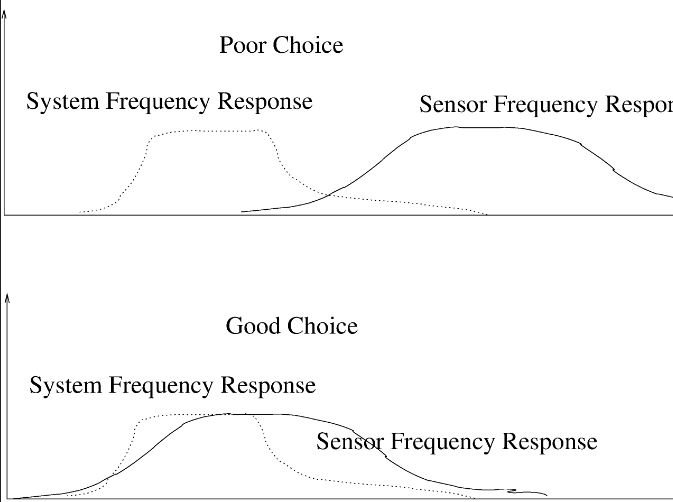
\includegraphics[scale=0.60]{day3_seg1_numerical/sensor_selection.jpg}
\end{frame}

\begin{frame}
  \onslide<1->{
	\frametitle{Kalman Filter Theory vs. Reality} 
	\framesubtitle{}
}
\begin{itemize}
  \onslide<2->{
  \item Choose sensors to match states.\\
E.g., consider the state model
\[
\begin{bmatrix}
\dot{x}_1\\
\dot{x}_2
\end{bmatrix}
= \begin{bmatrix}
0\\
0
\end{bmatrix}
\]
with the measurement model
\[
z = \begin{bmatrix} 1\;\; 0 \end{bmatrix}\begin{bmatrix}
x_1\\
x_2
\end{bmatrix}
+ v
\]
}
  \onslide<3->{
\item   Here $x_1$ is observable but $x_2$ is not, because there are no dynamic paths in $A=I$ flow infomation 
about $x_1$ into $x_2$
}
\end{itemize}
\end{frame}

\begin{frame}
  \onslide<1->{
	\frametitle{Kalman Filter Theory vs. Reality} 
	\framesubtitle{Sensor Selection}
}
\begin{itemize}
  \onslide<2->{
  \item Examine the $H$ matrix that you would use with this sensor!
}
  \onslide<3->{
  \item If it renders some states unobservable, then consider adding 
  additional sensors for those states, or replacing this sensor with one that is more favorable
}
\end{itemize}
\end{frame}
% day3_seg4_ins_challenges/observability.tex
\begin{frame}
  \onslide<1->{
	\frametitle{Observability} 
	\framesubtitle{}
}
\begin{itemize}
  \onslide<2->{
 \item Structural observability is concerned with how $H$ maps measurements into states
}
  \onslide<3->{
  \item Observability means there is a linear path from the measurements to states
}
  \onslide<4->{
  \item Structural observability determined by $\Phi$ and $H$:
}
  \onslide<5->{
\item  If $H$ is $1\times n$, where $n$ is the size of the state vector, then the state $x_0$ 
is said to be \textbf{observable }from $n$ scalar measurements $\set{z_0,\ldots,z_{n-1}}$ if the block matrix
\[
\begin{bmatrix}
H\trans&\Phi\trans H\trans & \cdots & (\Phi\trans)^{n-1}H\trans
\end{bmatrix}
\]
is of rank $n$

}
  \onslide<6->{
 \item Will making measurements as governed by $H$ actually enable us to estimate all of the states 
 in the state vector? 
}
 \end{itemize}
\end{frame}

\begin{frame}
  \onslide<1->{
	\frametitle{Observability} 
	\framesubtitle{Designing Observability into the Filter}
}
\begin{itemize}
  \onslide<2->{
  \item Observability challenge for filters is often a matter of choosing right kinds of sensors
}
  \onslide<3->{
  \item Choosing the right measurement scheduling
}
  \onslide<4->{
  \item Certain kinds of divergence can be the result of poor observability
}
  \onslide<5->{
\item   Example: Let $H=\left[1\;\;0\;\; 0\;\; 0\;\; 0\right]$, 
$\Phi=
\begin{bmatrix}
0&1&0&0&0\\
0&0&1&0&0\\
0&0&0&1&0\\
0&0&0&0&1\\
1& 2&3&4&5
\end{bmatrix}$
}
  \onslide<6->{
	\item What is the rank 
	of $\left[H\trans\;\;\Phi H\trans\;\;\Phi^2 H\trans\;\; \Phi^3 H\trans\;\;\Phi^4 H\trans\right]$?
}
\end{itemize}
\end{frame}



% day2_seg4_numerical/divergence.tex
\begin{frame}
  \onslide<1->{
	\frametitle{Filter Divergence} 
	\framesubtitle{}
}
\begin{itemize}
  \onslide<2->{
\item Kinds of Divergence
}
  \onslide<3->{
\item Causes and Remedies
}
\end{itemize}
\end{frame}

\begin{frame}
  \onslide<1->{
	\frametitle{Filter Divergence} 
	\framesubtitle{Kinds of Divergence}
}
\begin{itemize}
  \onslide<2->{
\item Mean estimation error is supposed to converge to 0
\begin{itemize}
	\item $\esterrdef$
	\item $\expect{\esterr}\rightarrow 0$
	\item Estimate is unbiased: $\expect{\hat{x}(k)}=x(k)$
\end{itemize}
}
  \onslide<3->{
\item Covariance matrix for estimation error is same as state estimation error covariance matrix: $\covmatdef$
}
\end{itemize}
\end{frame}

\begin{frame}
  \onslide<1->{
	\frametitle{Kinds of Divergence} 
	\framesubtitle{}
}
\begin{itemize}
  \onslide<2->{
\item For optimal filter, $P$ will indicate convergence or divergence.
	\begin{itemize}
		\item One common form of divergence due to round-off will send $P$ to zero
	\end{itemize}
}
  \onslide<3->{
\item For suboptimal filters, $P$ will not necessarily indicate divergence
	\begin{itemize}
	  \item $P$ may seem to indicate nominal steady-state values and yet the state estimate may go diverge from the true value
	\end{itemize}
}
\end{itemize}
\end{frame}


\begin{frame}

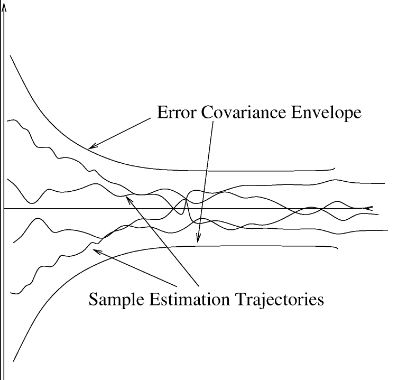
\includegraphics[scale=0.60]{day3_seg1_numerical/covconverge.jpg} 

\end{frame}


\begin{frame}
  \onslide<1->{
	\frametitle{Kinds of Divergence} 
	\framesubtitle{}
}
\begin{itemize}
  \onslide<2->{
\item Going to sleep:  error covariance becomes so small that measurements are no longer believed by the filter
}
  \onslide<3->{
\item Loss of symmetry in $P$
}
  \onslide<4->{
\item Loss of positive definiteness: negative numbers on the diagonal!
}
\end{itemize}
\end{frame}

% day2_seg4_numerical/numstab.tex
\begin{frame}
  \onslide<1->{
	\frametitle{Numerical Stability} 
	\framesubtitle{}
}
\begin{itemize}
  \onslide<2->{
 \item System stability:  Bounded input results in bounded output
}
  \onslide<3->{
 \item Numerical stability: small errors at each computation step do not grow without bound
}
  \onslide<4->{
 \item Matrix Conditioning (will address in discussing SRIF)
}
\end{itemize}
\end{frame}

%\input{day2_seg4_numerical/matrix_conditioning.tex}
% day2_seg4_numerical/roundoff.tex
\begin{frame}
  \onslide<1->{
	\frametitle{Round-Off Errors} 
	\framesubtitle{Joseph Form}
}
\begin{itemize}
  \onslide<2->{
 \item Computer round-off in floating point arithmetic
}
  \onslide<3->{
 \item Unit round-off value is largest number $\eps$ such that $1+\eps=1$
}
  \onslide<4->{
 \item In Matlab, the global symbol "eps" stores the unit round-off value
}
  \onslide<5->{
  \item Round-off errors generally plague the classical covariance update algorithm
\[\covupdateeq\]
\begin{itemize}
  \item Alternative, called the Joseph form, is more robust:
\[\josephcovupdateeq\]
\end{itemize} 
}
\end{itemize}
\end{frame}

\begin{frame}
  \onslide<1->{
	\frametitle{Round-Off Errors} 
	\framesubtitle{De Vries Mechanization}
}
\begin{itemize}
  \onslide<2->{
\item   This form in turn leads to the De Vries mechanization of the
Kalman gain equation.  To see this, first expand
the Joseph form (omitting subscripts for clarity):

}
  \onslide<3->{
\begin{align*}
   P(+)&= P(-)-KHP(-)-P(-)H\trans K\trans+ KHP(-)H\trans K\trans +
   KRK\trans.
\end{align*}
}
\end{itemize}
\end{frame}

\begin{frame}
  \onslide<1->{
	\frametitle{Round-Off} 
	\framesubtitle{De Vries}
}
\begin{itemize}
  \onslide<2->{
\item   Define
\begin{equation}\label{Feq}
  F=PH\trans
\end{equation}
and
\begin{equation}\label{Deq}
  D=HF+R.
\end{equation}

}
  \onslide<3->{
\item   We note that $D$ is symmetric, because
\begin{align*}
  D\trans &= [HF+R]\trans \\
  &= [HPH\trans + R]\trans \\
  &= [HPH\trans] \trans + R\trans \\
  &= [H\trans]\trans P\trans H\trans + R\trans \\
  &= HPH\trans + R & \text{(because $P$ and $R$ are symmetric)}\\
  &= HF + R \\
  &= D.
\end{align*}
}
\end{itemize}
\end{frame}

\begin{frame}
  \onslide<1->{
	\frametitle{Round-Off} 
	\framesubtitle{De Vries}
}
\begin{itemize}
  \onslide<2->{
\item   The gain in standard Kalman gain equation
\[\kalgaineq\] can be written as
\[K=FD^{-1}.\]
}
  \onslide<3->{
\item   Using Eqs.~(\ref{Feq}) and ~(\ref{Deq}), we compute
\begin{align*}
  P(+) &= P(-) - KF\trans - FK\trans + KDK\trans \\
  &= P(-)-K\left[F\trans - \frac{DK\trans}{2} \right] - \left[
  F-\frac{KD}{2}\right]K\trans.
\end{align*}

}
  \onslide<4->{
\item   Letting $G=F-\dfrac{KD}{2}$, we obtain
\begin{equation}\label{dvcovupdateeq}
  \dvcovupdateeq.
\end{equation}

}
\end{itemize}
\end{frame}

\begin{frame}
  \onslide<1->{
	\frametitle{Round-Off} 
	\framesubtitle{De Vries}
}
\begin{itemize}
  \onslide<2->{
\item   The De Vries mechanization implements Eq.~(\ref{dvcovupdateeq}) by
subtracting the $ij^{th}$ element of $GK\trans$ from both the
$ij^{th}$ and $ji^{th}$ elements of $P(-)$. 
}
  \onslide<3->{
\item   The De Vries form of
the covariance update equation is valid for any arbitrary gain
matrix $K$, not just the optimal gains computed from
Eqs.~(\ref{Feq}) and (\ref{Deq}).

}
\end{itemize}
\end{frame}

% day2_seg4_numerical/matinv.tex
\begin{frame}
  \onslide<1->{
	\frametitle{Numerical Stability} 
	\framesubtitle{Matrix Inversion}
}
\begin{itemize}
  \onslide<2->{
 \item Matrix inversion is always risky due to potential ill-conditioning
}
  \onslide<3->{
 \item One way to avoid this is to process measurements sequentially as scalars
}
  \onslide<4->{
 \item Or at least as low-dimensional matrices
}
\end{itemize}
\end{frame}

%% day2_seg4_numerical/symmloss.tex
\begin{frame}
Loss of Symmetry and Positive Definiteness
 \begin{itemize}
 \item
 \item
 \item
\end{itemize}
\end{frame}

% day2_seg4_numerical/exercises.tex
\begin{frame}
  \onslide<1->{
	\frametitle{Exercises} 
}
\begin{itemize}
  \onslide<2->{
\item   1. Let $v=[1\;\; -2]\trans$.  Compute the positive definite, symmetrix matrix $M=vv\trans$

}
  \onslide<3->{
\item   2. Use the following algorithm (Grewal \& Andrews) to factor $M$ into $UDU\trans$ form:
}
\end{itemize}
\end{frame}
\begin{frame}[fragile]
	\frametitle{Exercises} 
\begin{verbatim}
for j=m:-1:1
    for i=j:-1:1
        covar=P(i,j);
        for k=j+1:m
            covar=covar-U(i,k)*D(k,k)*U(j,k);
        end
        if i==j
            D(j,j)=covar;
            U(j,j)=1;
        else
            U(i,j)=covar/D(j,j);
        end
    end
end
\end{verbatim}
\end{frame}


\section{Square Root Information Filer (SRIF)}
\subsection{SRIF Topics}
\begin{frame}
  \onslide<1->{
	\frametitle{Square Root Information Filters} 
	\framesubtitle{Topics}
}
\begin{itemize}
  \onslide<2->{
\item  Information Filters 
}
  \onslide<3->{
\item  Square Root Filters 
}
  \onslide<4->{
\item  Square Root Information Filters (SRIF) 
}
\end{itemize}
\end{frame}


\subsection{Information Filters}
\begin{frame}
  \onslide<1->{
	\frametitle{Square Root Information Filters} 
	\framesubtitle{Information Filters}
}
\begin{itemize}
  \onslide<2->{
\item Standard KF is sometimes called the Covariance Kalman Filter because it is formulated
using the covariance matrix $P$.  The Information Filter is more efficient when there are very large batches of 
measurements to process.
}

  \onslide<3->{
\item Information Matrix $\Lambda$:  Inverse of the Estimation Error Covariance Matrix $P$  \\
}
  \onslide<4->{
\item Recall $\gencovmatdef$  
}
  \onslide<5->{
\item  We define $\Lambda:=P^{-1}$ 
}
  \onslide<6->{
\item When $\Lambda$ is "large" $P$ is "small" (in norm)  
}
\end{itemize}
\end{frame}
\begin{frame}
  \onslide<1->{
	\frametitle{Square Root Information Filters} 
	\framesubtitle{Information Filters}
}
\begin{itemize}
  \onslide<2->{
\item  Consider the covariance update equation $\gencovupdateeq$ 
}
  \onslide<3->{
  % Taking inverses yields:  $\left[P^{+}\right]^{-1}=\left[P^{-}\right]^{-1}\left[ I-KH\right]^{-1}$ 
\item  Substitute the Kalman gain formula $\genkalgaineq$ into the above equation to yield\\
$P^{+}=P^{-}-P^{-}H\trans\left[HP^{-}H\trans+R\right]^{-1}HP^{-}$  
}
  \onslide<4->{
\item   To futher expand and then simplify, we need to apply the Matrix Inversion Lemma (also known as the Woodbury formula):\\
$\woodbury{A}{B}{C}{D}$
}
  \onslide<5->{
\item We obtain:  $\left[P^{+}\right]^{-1}=\left[P^{-}\right]^{-1}+H\trans R^{-1}H$, or,\\ in terms of $\Lambda$:
$\Lambda^{+}=\Lambda^{-}+H\trans R^{-1}H$  
}
\end{itemize}
\end{frame}

\begin{frame}
  \onslide<1->{
	\frametitle{Square Root Information Filters} 
	\framesubtitle{Information Filters}
}
\begin{itemize}
  \onslide<2->{
\item  Note that the information matrix is updated without knowledge of the gain!
}
  \onslide<3->{
\item  The gain comutation takes on a very simple form:  $K=\Lambda^{+}H\trans R^{-1}$  
}
  \onslide<4->{
\item  The state is then updated using the gain in the normal way 
}
  \onslide<5->{
\item  Standard KF requires inversion of $r\times r$ matrix ($r=$number of measurements); information filter
requires inversion of a couple of $n\times n$ inversions.   \\
Thus, if $r>>n$, it is more efficient to use the information filter.
}
\end{itemize}
\end{frame}
\begin{frame}
  \onslide<1->{
	\frametitle{Square Root Information Filters} 
	\framesubtitle{Information Filters}
}
\begin{itemize}
  \onslide<2->{
\item  The information matrix extrapolation equation is derived in a similar fashion by 
transforming the standard covariance extrapolation equation using once again the Woodbury formula
}
  \onslide<3->{
\item  This yields:\\ $\Lambda^{-}(k)=Q^{-1}-Q^{-1}\Phi\left[ \Lambda^{+}(k-1)+\Phi\trans Q^{-1} \Phi\right]^{-1}\Phi\trans Q^{-1}$ 
}
  \onslide<4->{
\item   If the process noise covariance $Q$ and/or the measurement noise covariance are constant (
or change only infrequently) with time, then the indicated inverses can be computed once at startup or perhaps only 
occasionaly.
}
\end{itemize}
\end{frame}

\subsection{Square Root Filters}
\begin{frame}
  \onslide<1->{
	\frametitle{Square Root Information Filters} 
	\framesubtitle{Square Root Filters}
}
\begin{itemize}
  \onslide<2->{
\item Motivation: Covariance matrices are supposed to be nonsingular, positive semi-definite; they are invertible  
}
  \onslide<3->{
\item  But due to differences in uncertainy values for different states, they may be ill-conditioned for inversion 
}
  \onslide<4->{
\item  Conditioning refers to the condition number of a matrix:  $\kappa (P):=\sigma_{\text{max}}/\sigma_{\text{min}}$,\\
where $\sigma_{\text{max}}$ is the maximum singular value of $P$ and $\sigma_{\text{min}}$ is the minimum singular value.\\
\begin{footnotesize} 
Singular values of real-valued $P$ are square roots of eigenvalues of $P\trans P$ (or $PP\trans$)
\end{footnotesize}
}
  \onslide<5->{
\item  Note that $\kappa(P)\geq 1$, for a nonsingular matrix $P$, since all of its singular values are positive
}
\end{itemize}
\end{frame}

\begin{frame}
  \onslide<1->{
	\frametitle{Square Root Information Filters} 
	\framesubtitle{Square Root Filters}
}
\begin{itemize}
  \onslide<2->{
\item Example of 2-state model: Highly uncertain first state, but highly certain second state:\\
$P=
\begin{bmatrix}
10^{10} & 0\\
0 & 10^{-10}
\end{bmatrix}$  
}
  \onslide<3->{
\item $\kappa(P)=10^{10}/10^{-10}=10^{20}$, since singular values of a diagonal matrix 
are absolute values of the diagonal elements  
}
  \onslide<4->{
\item Although $P$ is technically nonsingular, on an embedded digital computer with limited word length 
it may become singular   
}
  \onslide<5->{
\item  MATLAB Warning: Matrix is close to singular or badly scaled. Results may be inaccurate. RCOND =
1.000000e-20 
}
\end{itemize}
\end{frame}

\begin{frame}
  \onslide<1->{
	\frametitle{Square Root Information Filters} 
	\framesubtitle{Square Root Filters}
}
\begin{itemize}
  \onslide<2->{
\item If we can factor $P$ as the product of a matrix and its transpose, i.e., $P=SS\trans$, then the matrix $S$  
is said to be the matrix square root of $P$\\
\begin{footnotesize}Note: There are several alternative definitions in the literature $SS\trans,S^2,S\trans S$\end{footnotesize}
}
  \onslide<3->{
\item Key idea:  if $P=SS\trans$, then $\kappa(S)=\sqrt{\kappa(P)}$  
}
  \onslide<3->{
\item Matrix square roots are not unique  
}
  \onslide<4->{
\item But all square roots of a matrix are related by orthogonal transformations (i.e., 
rotations in n-dimensional space)\\
$T$ is \textbf{orthogonal} if its transpose is its inverse:   $TT\trans = T\trans T=I$  
}
  \onslide<5->{
\item If $P=S_1 S_1\trans=S_2 S_2\trans$, then there is an orthogonal matrix $T$ such that $S_2=S_1 T$
}
\end{itemize}
\end{frame}

\begin{frame}
  \onslide<1->{
	\frametitle{Square Root Information Filters} 
	\framesubtitle{Square Root Filters: Orthogonal Matrices}
}
\begin{itemize}
  \onslide<2->{
\item Important Properties of Orthogonal Matrices:  
}
\begin{itemize}
  \onslide<3->{
\item Length Invariance (Isometry):  $\norm{Tx}=\norm{x}$  \\
where $\norm{x}=\sqrt{x\trans x}$ is Euclidean norm\\ (also preserves dot product between two vectors)
}
  \onslide<4->{
\item Angle Invariance:  The angle between the vectors $x$ and $y$ is the same as that between $Tx$ and $Ty$ 
}
  \onslide<5->{
\item  Standard Gaussian Invariance: If $v$ is zero-mean Gaussian random vector such that $\expect{vv\trans}=I$, 
then for orthogonal $T$ the 
vector $Tv$ is also zero-mean Gaussian and $\expect{Tv(Tv)\trans}=I$
}
\end{itemize}
  \onslide<6->{
    \item Length and Standard Gaussian Invariances play crucial role in square root filtering
}
\end{itemize}
\end{frame}

\subsection{Bierman Derivation of SRIF}
\begin{frame}
  \onslide<1->{
	\frametitle{Square Root Information Filters} 
	\framesubtitle{Least Squares Derivation of SRIF (Bierman)}
}
\begin{itemize}
  \onslide<2->{
\item Consider measurement model:  $z=Hx+v$  
}
  \onslide<3->{
\item  Least squares solution minimizes means square error:  $$J=\sum_{j=1}^m v^2(j)=v\trans v$$ 
}
  \onslide<4->{
\item As a function of $x$ this becomes $$J(x)=(z-Hx)\trans (z-Hx)$$  
}
\end{itemize}
\end{frame}

\begin{frame}
  \onslide<1->{
	\frametitle{Square Root Information Filters} 
	\framesubtitle{Least Squares Derivation of SRIF (Bierman)}
}
\begin{itemize}
  \onslide<2->{
\item  Differentiating $J(x)$ with respect to $x$ (taking into account non-commutative multiplication of matrices),
we obtain the least squares \textbf{normal equations}: $$H\trans H x=H\trans z$$
}
  \onslide<3->{
\item  The least squares solution $x_{\text{ls}}$ is therefore $$x_{\text{ls}}=(H\trans H)^{-1}H\trans z$$ 
}
\end{itemize}
\end{frame}

\begin{frame}
  \onslide<1->{
	\frametitle{Square Root Information Filters} 
	\framesubtitle{Least Squares Derivation of SRIF (Bierman)}
}
\begin{itemize}
  \onslide<2->{
\item   Interpreting the errors $v$ statistically and assuming both $\expect{v}=0$ and $\expect{vv\trans}=I$,
we derive $$H\trans H \left(x_{\text{ls}}-x\right)=H\trans v$$
}
  \onslide<3->{
\item  And it can be shown that $$P_{\text{ls}}=(H\trans H)^{-1}$$ 
}
  \onslide<4->{
\item  Taking the matrix inverse of both sides reveals SRI matrix $$\Lambda_{\text{ls}} = H\trans H$$ 
}
\end{itemize}
\end{frame}

\begin{frame}
  \onslide<1->{
	\frametitle{Square Root Information Filters} 
	\framesubtitle{Least Squares Derivation of SRIF (Bierman)}
}
\begin{itemize}
  \onslide<2->{
\item  The above derivation was \textit{a posteriori}, i.e., after the measurement
}
  \onslide<3->{
\item  We can now incorpoate the \textit{a priori} estimate $\hat{x}^{-}$ and SRI matrix $\Lambda^{-}$
}
  \onslide<4->{
\item  The previous performance functional is now modified to become
$$
J_1(x):=(x-\hat{x}^{-})\trans \Lambda^{-} (x-\hat{x}^{-})+(z-Hx)\trans (z-Hx)
$$
}
\end{itemize}
\end{frame}

\begin{frame}
  \onslide<1->{
	\frametitle{Square Root Information Filters} 
	\framesubtitle{Least Squares Derivation of SRIF (Bierman)}
}
\begin{itemize}
  \onslide<2->{
\item  The vector that minimizes $J_1$ is denoted $\hat{x}^{+}_{\text{ls}}$ and is easily shown to satisfy
$$
(\Lambda^{-}+H\trans H)\hat{x}^{+}_{\text{ls}}=\Lambda^{-}\hat{x}^{-}+H\trans z
$$

}
  \onslide<3->{
\item   Finally, the updated covariance is
$$
P^{+}_{\text{ls}}=(\Lambda^{-}+H\trans H)^{-1}
$$
}
  \onslide<4->{
\item  Bierman points out that $\Lambda^{-}$ need not be non-singular
}
  \onslide<5->{
\item  In fact, one of the advantages of using the information matrix instead of the covariance 
is that many entries of $\Lambda^{-}$ may be 0 (meaning no information=infinite uncerrtainty); we 
may even start with $\Lambda^{-}=0$
}
\end{itemize}
\end{frame}

\begin{frame}
  \onslide<1->{
	\frametitle{Square Root Information Filters} 
	\framesubtitle{SRIF Recursion (Bierman)}
}
\begin{itemize}
  \onslide<2->{
\item Factor the \textit{a priori} $\Lambda^{-}$ into square root factors:  
$\Lambda^{-}=\left[S^{-}\right]\trans S^{-}$
}
  \onslide<3->{
\item This allows us to rewrite first term of $J_1(x)$ as
$$
(x-\hat{x}^{-})\trans \Lambda^{-} (x-\hat{x}^{-})=(z^{-}-S^{-}x)\trans (z^{-}-S^{-}x)
$$
where $z^{-}= S^{-}x^{-}$
}
  \onslide<4->{
\item  We can now treat the \textit{a priori} estimate and covariance information 
as if they were an additional (pseudo) measurement and augment the least squares problem
$$
\begin{bmatrix}
z^{-}\\
z
\end{bmatrix}
=
\begin{bmatrix}
S^{-}\\
H
\end{bmatrix}
x +
\begin{bmatrix}
v^{-}\\
v
\end{bmatrix}
$$
}
\end{itemize}
\end{frame}

\begin{frame}
  \onslide<1->{
	\frametitle{Square Root Information Filters} 
	\framesubtitle{Summary}
}
\begin{itemize}
  \onslide<2->{
\item  Bierman:  "The interpretation of the \textit{a priori} as additional observations is the cornerstone
of the square root information filter." 
}
  \onslide<3->{
\item  Results do not depend on which square root is used;  facilitates use of orthogonal transformations 
(Householder, Givens matrices) to put the square roots into numerical convenient forms 
}
  \onslide<4->{
\item   Bierman and Thornton (JPL) combined this SRIF formulation with Cholesky decomposition to devise the U-D 
factorization
}
\end{itemize}
\end{frame}
\begin{frame}
  \onslide<1->{
	\frametitle{UD Factorization} 
	\framesubtitle{Bierman and Thornton}
}
\begin{itemize}
  \onslide<2->{
  \item Based on Cholesky Decomposition
}
  \onslide<3->{
  \item Unit Triangular Matrices: $U$ has 1's on the diagonal and all 0's below the diagonal.  E.g.,
\[
U=\begin{bmatrix}
1 & 5 & 7 \\
0 & 1 & 3\\
0 & 0 & 1
\end{bmatrix}
\]
}
\end{itemize}
\end{frame}

\begin{frame}
  \onslide<1->{
	\frametitle{UD Factorization} 
	\framesubtitle{}
}
\begin{itemize}
  \onslide<2->{
  \item Factor $P^{-}$ as $UDU\trans$, where $U$ is unit upper triangular and $D$ is diagonal.
}
  \onslide<3->{
  \item This then allows us to "invert" $P^{-}$ by solving the equation unit upper triangular equation $UDU\trans X=H$ for the matrix $X$, which will yield $X=\left[HPH\trans + R\right]^{-1}H$
}
  \onslide<4->{
  \item This last expression is used on the covariance update equation in $KH$
}
\end{itemize}
\end{frame}



\section{Navigation Applications}
\begin{frame}
\frametitle{Overview}
\begin{itemize}
  \item Etymology of the term 'Navigation':  Latin $navis$='ship' and $agere$='to move or direct'
  \item Arose out of marine or ship navigation due to the challenge of navigating without landmarks
  \item Modern distinction between navigation and guidance
  \begin{itemize}
    \item navigation associated with state determination (open loop)
    \item guidance associated with control feedback (closed loop)
  \end{itemize} 
\end{itemize} 
\end{frame}

\begin{frame}
  \frametitle{The Navigation Problem from a Mathematical Perspective}
With respect to some mathematical reference frame, determine ...
\begin{itemize}
  \item vector displacement (3d position) and its time derivatives (velocity, acceleration, ...)
  \item rotational orientation (3d attitude) and its time derivatives (angular velocity, angular acceleration, ...) 
  \item Note:  This is a pure mathematics problem ... sensors do not enter into it
\end{itemize} 
\end{frame}


\begin{frame}
  \frametitle{The Navigation Problem from a Mathematical Perspective}
\begin{itemize}
  \item Reference frame is crucial:
  \begin{itemize}
    \item Position:  origin and three linearly independent vectors yields three numbers
    \item Attitude:  rotations about three linearly indepedent vectors yields three numbers
  \item I.e., 6 DOF = six degrees of freedom (3 position coordinates + 3 attitude coordinates)
  \end{itemize}
\end{itemize} 
\end{frame}


\begin{frame}
 \frametitle{The Navigation Problem from a Real World Physical Perspective}
\begin{itemize}
  \item Which reference frame should we use?
  \item Rectilinear or curvilenar coordinate system?
\end{itemize} 
\end{frame}

\begin{frame}
 \frametitle{The Navigation Problem from a Real World Physical Perspective}
\framesubtitle{Position}
For terrestrial navigation, global spherical (spheroidal) coordinates are used:
\begin{itemize}
  \item Latitude:  $\pm 90$ degrees north(+) or south(-) of the equator.
  \item Longitude: $\pm 180$ degrees east(+) or west(-) of the prime meridian through Greenwich, England
  \item Height:  Above the ellipsoid (normal to surface), or radius from center of earth
\end{itemize} 
\end{frame}

\begin{frame}
 \frametitle{The Navigation Problem from a Real World Physical Perspective}
\framesubtitle{Direction:  Bearing, Course, Track}
\begin{itemize}
  \item North Reference:  True and Magnetic. Direction angles are usually referenced clockwise with respect to north.
  \item  Bearing:  The angle with respect to north from one point on earth to another
  \item  Track:    The angle made by velocity vector with respect to north
  \item  Course:   Sometimes used synonym for track; sometimes expresses desired track vs. actual track
  \item  Heading:  Direction vehicle is pointing in with respect to north
\end{itemize} 
\end{frame}

\begin{frame}
 \frametitle{The Navigation Problem from a Real World Physical Perspective}
\framesubtitle{The Need for Sensors}
\begin{itemize}
  \item Reference frames are necessary, but not sufficient for real world navigation
  \item Also need real world sensor measurement data indicative of locations, distances, angles, etc. with respect to these reference frames
  \item But real world sensors are not perfect!  They only provide apparent positions, distances, angles, etc.
\end{itemize} 
\end{frame}

% day3_seg1_navproblem/navproblem_main.tex
\begin{frame}
\frametitle{\textbf{The Navigation Problem and Reference Frames}}
\framesubtitle{Topics}
 \begin{itemize}
 \item Basic Navigation Problem and Solutions
 \item Earth Referenced Navigation
 \item Coordinate Frame Conversion
 \item Basic Strapdown Navigation Equations
\end{itemize}
\end{frame}

% day3_seg1_navproblem/basicnavprob.tex
%\begin{frame}
%Solutions to the Basic Navigation Problem\\
%Solution in Inertial Space
% \begin{itemize}
% \item In an inertial reference frame, it's no problem, if you 
% have a cluster of inertial sensors and you know your initial 
% position:
% \item Just integrate the acceleration once to get velocity, 
%twice to get
% position.
%\[v(T) = v(0) + \int_{0}^{T}\dfrac{d^2r}{dt^2}dt\]
%\[r(T) = r(0) + \int_{0}^{T}v(t)dt\]
% \item And integrate the angular rate once to get attitude.
%\end{itemize}
%\end{frame}

%\begin{frame}
%Solution in Inertial Space
%\begin{itemize}
%  \item Solution easy in inertial space because ...
%  \begin{itemize}
%	\item inertial instruments sense acceleration and rotational % rate with respect to inertial coordinate frame 
%	\item inertial frame attached to sensor platform
%    \item Note: You still need to rotate accelerations from body %to inertial coordinates prior to integration (strapdown)
%  \end{itemize}
%  \item But we don't necessarily want the answer to our 
%questions expressed in terms of inertial coordinates!
%\end{itemize} 
%\end{frame}

\begin{frame}
\frametitle{Dead Reckoning}
\begin{itemize}
  \item Process of determining new position based on extrapolating from previously known position and velocity.
  \item Velocity = Speed and Direction
  \item Unaided inertial navigator is essentially a dead reckoning computer
\end{itemize} 
\end{frame}






% day3_seg1_navproblem/earthrev.tex
\begin{frame}
\frametitle{Earth Referenced Navigation}
 \begin{itemize}
 \item Terrestial navigation seeks to answer nav questions with respect to earth
 \begin{itemize}
   \item Global earth reference
   \item Local or relative navigation
 \end{itemize}
 \item Complications:
 \begin{itemize}
   \item Earth surface is curved (ellipsoid)
   \item Earth is turning (can usually ignore motion about the Sun for terrestrial nav)
 \end{itemize}
\end{itemize}
\end{frame}

\begin{frame}
\frametitle{Earth Model:  WGS 84}
\begin{itemize}
  \item Earth is not spherical, but oblate spheroid or ellipsoid
  \item Flattened at the poles
  \item World Geodetic System 84:
  \begin{itemize}
   \item Semi-major axis:  6,378,137.0 m
        \item Semi-minor axis:  6,356,752.314  m
  \end{itemize}
  \item Not the same as geoid:  no terrain or gravity model
\end{itemize} 
\end{frame}

% day3_seg1_navproblem/coordconv.tex
\begin{frame}
\frametitle{Coordinate Frames}
 \begin{itemize}
 \item Inertial
 \item Earth Fixed
 \item Local Level
 \item Body
\end{itemize}
\end{frame}
\begin{frame}
\frametitle{Coordinate Frames}
 \begin{itemize}
  \item Technically speaking, all frames are earth-centered
  \begin{itemize}
    \item Common origen needed for linear transformations (such as rotations)
    \item Can compensate by using a translation
  \end{itemize}
  \item Practically speaking, we think of the Body frame as centered in the body of the vehicle (usually at center of gravity).
  \item Local Level is thought to be located at surface of earth directly beneath the vehicle.
\end{itemize}
\end{frame}
\begin{frame}
\frametitle{Inertial Reference Frames}
 \begin{itemize}
 \item Non-Rotating
 \item Non-Accelerating
 \item Fixed or moving uniformly with respect to another inertial
 frame (fixed stars)
\end{itemize}
\end{frame}

\begin{frame}
\frametitle{Inertial Reference Frames}
 \begin{itemize}
 \item Nav problem "easy" in inertial frames
 \item Integrate gyro rates once to get attitude (rotational motion independent of lateral motion)
 \item Rotate accelerometer outputs to inertial frame using attitude matrix, then integrate to get inertial
 velocity; integrate velocity to get position.
 \item Would still have to contend with instrument imperfections.
\end{itemize}
\end{frame}

\begin{frame}
\frametitle{Inertial Reference Frame Integrations}
\begin{equation}\label{inertacceleq}
\ddot{r}(t)=\specforce+\text{other external forces}
\end{equation}
\begin{equation}\label{inertveleq}
v(T)=\dot{r}(T)=v(0)+\int_{0}^{T}\specforce dt + \int_{0}^{T}(\text{other
external forces})dt
\end{equation}
\begin{equation}\label{inertposeq}
  r(T)=r(0)+\int_{0}^{T}v(t)dt
\end{equation}
\end{frame}

\begin{frame}
\frametitle{Earth Fixed = ECEF = Earth Centered Earth Fixed}
 \begin{itemize}
 \item Rotating frame, i.e., non-inertial
 \item Cartesian ($X,Y,Z$ in meters)
 \item Spherical (latitude $\lat$, longitude $\lon$, altitude $\alt$)
 \begin{itemize}
 \item geodetic
 \end{itemize}
\end{itemize}
\end{frame}


\begin{frame}
\frametitle{Local Level}
 \begin{itemize}
 \item Tangent to earth's surface but translated to center of
 earth.
 \item Vertical $Z$-axis is normal to earth's surface
 \item $X,Y$-axes are level
 \item Several kinds: $Y$ north-slaved, wander (0 transport rate) or free azimuth
 \item $Y$ makes wander angle $\alpha$ with respect to true north (ENU=East, North, Up).
\end{itemize}
\end{frame}

\begin{frame}
\frametitle{Earth Centered, Earth Fixed:  ECEF}
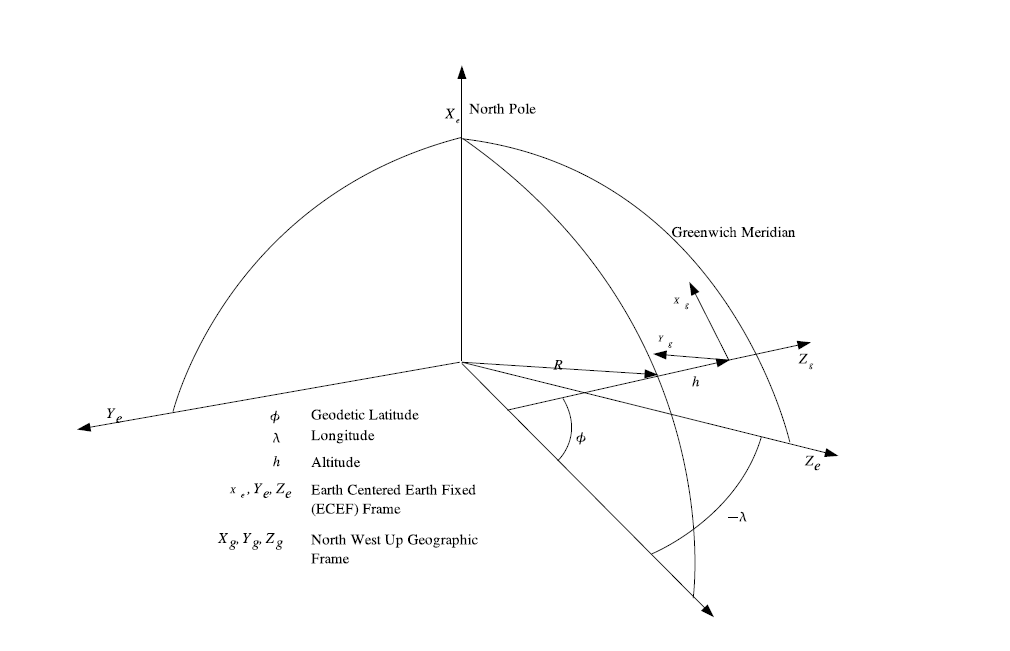
\includegraphics[width=\textwidth]{graphics/ecef.png}
\vfill
\end{frame}


\begin{frame}
\frametitle{Body Frame}
 \begin{itemize}
 \item Attached to vehicle
 \item For aircraft:
   \begin{itemize}
    \item $X$ out the nose
    \item $Y$ out the right wing
    \item $Z$ down
   \end{itemize}
\end{itemize}
\end{frame}

\begin{frame}
\frametitle{Body Frame (cont)}
 \begin{itemize}
 \item For space vehicles RIC:
   \begin{itemize}
    \item $R$ downward on radius to center of earth
    \item $I$ in-track, in direction of motion
    \item $C$ cross-track, perpendicular to motion
   \end{itemize}
 \item Also sometimes referred as RAC, where 'A' stands for 'along-track'
\end{itemize}
\end{frame}

\begin{frame}
\frametitle{Coordinate Frame Conversion}
 \begin{itemize}
 \item All frames earth-centered, differing only by
 rotation
 \item Rotation represented by direction cosine matrix (DCM) or set of four quaternions
 \begin{itemize}
	\item Expresses angles made by basis vectors of one frame with those of another
 \end{itemize}
 \item $\dcm{A}{B}$ = DCM transformation from frame A to frame B
\end{itemize}
\end{frame}

\begin{frame}
\frametitle{Coordinate Frame Conversion}
\begin{itemize}
  \item "Direction Cosine" comes from dot product:
\[\ip{x}{y}=x\cdot y=\norm{x}\norm{y}\cos\theta_{xy}\]
where $\theta_{xy}$ is the angle between the two vectors $x$ and $y$.
  \item If $x$ and $y$ are unit vectors, then $\norm{x}=\norm{y}=1$ and we have:
\[\ip{x}{y}=x\cdot y=\cos\theta_{xy}\]
\end{itemize} 
\end{frame}

\begin{frame}
\frametitle{Coordinate Frame Conversion}
\begin{itemize}
  \item If $U=\set{u_1,u_2,u_3}$ and $V=\set{v_1,v_2,v_3}$ are two sets of orthonormal basis vectors, then the DCM relating one frame to the other is given by:
\begin{align*}
\dcm{U}{V}&=
\begin{bmatrix}
\ip{u_1}{v_1} & \ip{u_1}{v_2} & \ip{u_1}{v_3}\\
\ip{u_2}{v_1} & \ip{u_2}{v_1} & \ip{u_2}{v_3}\\
\ip{u_3}{v_1} & \ip{u_3}{v_2} & \ip{u_3}{v_3}\\
\end{bmatrix}\\
&=
\begin{bmatrix}
\cos\theta_{11} & \cos\theta_{12} & \cos\theta_{13}\\
\cos\theta_{21} & \cos\theta_{22} & \cos\theta_{23}\\
\cos\theta_{31} & \cos\theta_{32} & \cos\theta_{33}\\
\end{bmatrix}
\end{align*}
\end{itemize} 
\end{frame}

\begin{frame}
\frametitle{Coordinate Frame Conversion}
\begin{itemize}
  \item If $V=\set{v_1,v_2,v_3}$ is considered to be the reference frame and its units vectors are the standard basis so that 
\[
v_1=\begin{bmatrix}
	1\\
	0\\
	0\\
	\end{bmatrix},
v_2=\begin{bmatrix}
	0\\
	1\\
	0\\
	\end{bmatrix},
v_3=\begin{bmatrix}
	0\\
	0\\
	1\\
	\end{bmatrix},
\]
then the DCM simplifies to just the coordinates of $u_1,u_2,u_3$ vectors with respect to $V$:
\begin{align*}
\dcm{U}{V}&=
\begin{bmatrix}
u_{11}& u_{12} & u_{13}\\
u_{21} & u_{22} & u_{23}\\
u_{31} & u_{32} & u_{33}\\
\end{bmatrix}
\end{align*}
\end{itemize} 
\end{frame}


\begin{frame}
\frametitle{Coordinate Frame Conversion}
 \begin{itemize}
 \item DCMs are (real) orthogonal matrices $\Rightarrow \left[\dcm{A}{B} \right]^{-1}=\left[\dcm{A}{B} \right]\trans=\dcm{B}{A}$
 \item Third row (or column) is vector cross product of other two\\
 $\Rightarrow$ only six independent parameters
 \item DCMs satisfy:   $\dcm{B}{A}\dcm{C}{B}=\dcm{C}{A}$
\end{itemize}
\end{frame}

\begin{frame}
\frametitle{Coordinate Frame Conversion}
 \begin{itemize}
 \item Orthogonal matrices preserve lengths of vectors: $\norm{Rx}=\norm{x}$
 \item Orthogonal matrices also preserve angles between vectors:  $\ip{Rx}{Ry}=\ip{R\trans Rx}{y}=\ip{Ix}{y}=\ip{x}{y}$
 \item Intuitively obvious in the case of rotations
\end{itemize}
\end{frame}

\begin{frame}
\frametitle{DCMs and Euler Rotation}
 \begin{itemize}
 \item Euler showed that three simultaneous rotations about three orthogonal axes can be
viewed as a single rotation about a single axis
 \item The single angle $\theta$ of rotation for a DCM can be determined from the eigenvalues of the DCM, which are:
\[
\set{1, \exp(i\theta), \exp(-i\theta)}
\]
\item The determinant of a DCM is therefore always 1.   Why? (Hint: How do you compute the determinant from the eigenvalues?)
\end{itemize}
\end{frame}

\begin{frame}
\frametitle{Euler Rotation}
\begin{figure}[h]
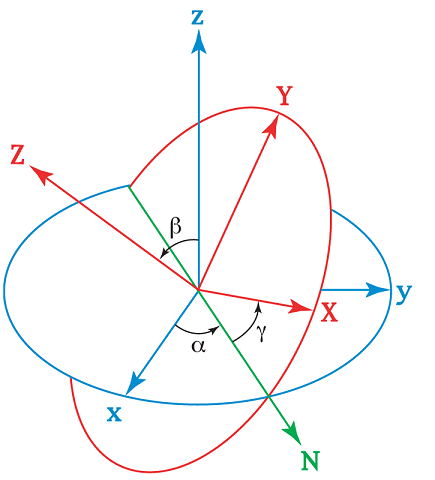
\includegraphics[width=0.5\textwidth]{graphics/euler.png}
\end{figure}
\end{frame}


\begin{frame}
\frametitle{DCMs and Euler Rotation}
 \begin{itemize}
 \item The axis of rotation for the single Euler rotation can be found from DCM as follows:
\begin{align*}
\dcm{U}{V}&=
\begin{bmatrix}
u_{11}& u_{12} & u_{13}\\
u_{21} & u_{22} & u_{23}\\
u_{31} & u_{32} & u_{33}\\
\end{bmatrix}
\end{align*}
then the axis of rotation $r = [r_1,r_2,r_3]\trans$ is given by
\begin{align*}
r_1 &= u_{12}u_{23} - (u_{22}-1)u_{13}\\
r_2 &= u_{21}u_{13} - (u_{11}-1)u_{23}\\
r_3 &= (u_{11}-1)(u_{22}-1) - u_{12}u_{21}\\
\end{align*}
\end{itemize}
\end{frame}

\begin{frame}
\frametitle{DCMs and Quaternions}
 \begin{itemize}
 \item If $C$ is a direction cosine matrix with elements $c_{ij}$, then the following four quantities define a quaternion of the rotation:
\begin{align*}
q_1 &= \dfrac{1}{4q_4}(c_{23}-c_{32})\\
q_2 &= \dfrac{1}{4q_4}(c_{13}-c_{31})\\
q_3 &= \dfrac{1}{4q_4}(c_{21}-c_{12})\\
q_4 &= \pm \dfrac{1}{2}\sqrt{1+c_{11}+c_{22}+c_{33}}\\
\end{align*}
\end{itemize}
\end{frame}

\begin{frame}
\frametitle{DCMs and Quaternions}
 \begin{itemize}
 \item It's even simpler to obtain quaternions from Euler rotation angle $\theta$ and axis given by a unit vector $u$:
\[q_i=u_i\sin(\theta/2), \text{ for } i=1,2,3\]
and
\[q_4=\cos(\theta/2)\]
\end{itemize}
\end{frame}


\begin{frame}
\frametitle{Coordinate Frame Conversion: Most important DCMs for terrestrial navigation}
 \begin{itemize}
 \item Body to Local Level: $\dcm{B}{L}$
 \begin{itemize}
 \item sometimes called Body to Nav and notated $\dcm{B}{N}$
 \item yields attitude info (Euler angles for roll, pitch, yaw)
 \end{itemize}
 \item Local Level to Earth: $\dcm{L}{E}$
 \begin{itemize}
 \item yields position info and also used to transform earth rate to
 local level
 \end{itemize}
\end{itemize}
\end{frame}
\begin{frame}
\frametitle{Coordinate Frame Conversion: Most important DCMs}
\begin{itemize}
  \item Visualize $\dcm{L}{E}$'s determination of position as follows:
	\begin{itemize}
		\item As vehicle moves, local level frame changes its orienation with respect to earth's center in order to maintain local level with respect to earth's surface
		\item If you think of local level frame as attached to earth's surface, you get distracted by the displacement of the frame
		\item If you move local level frame to center of earth, the displacement disappears and all that remains are the rotations
	\end{itemize} 
\end{itemize} 
\end{frame}

\begin{frame}
\begin{figure}
\centering
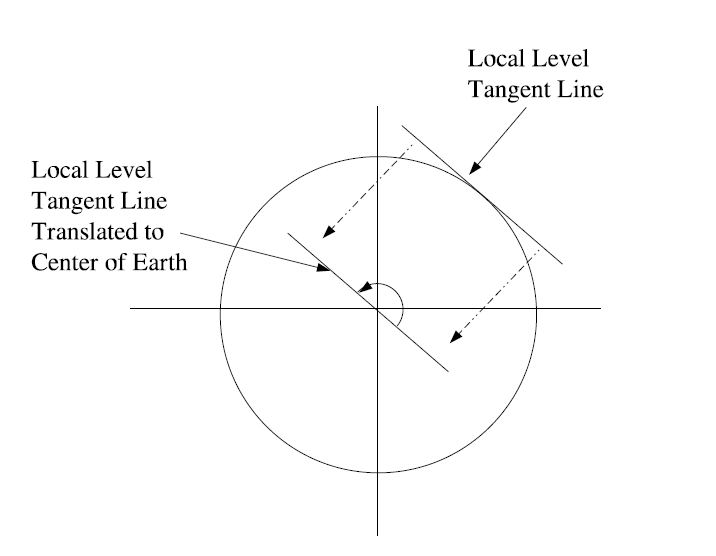
\includegraphics[width=\textwidth]{graphics/local_level.png}
\caption{Local Level to Earth Transformation}
\end{figure}
\end{frame}
% day3_seg1_navproblem/strapdown.tex
\begin{frame}
\frametitle{Inertial navigation Systems}
\framesubtitle{Strapdown Navigation:  Strapdown vs. Gimbaled}
\begin{itemize}
  \item Gimbaled INS:
  \begin{itemize}
	\item Gyro stabilized platform
	\item Gimbal assembly and torque motors
	\item Resolvers, slip rings, bearings, etc. to control  platform
	\item Goal: Maintain stable, locally level or inertial reference frame
  \end{itemize}
\end{itemize} 
\end{frame}


\begin{frame}
\frametitle{Strapdown Navigation: Strapdown vs. Gimbaled}
\begin{itemize}
  \item Gimbaled INS Issues
  \begin{itemize}
	\item Reliability and Cost: Lots of moving parts!
	\item Body rate and acceleration information not directly available
	\item Rate signals are generally noisy and have low bandwidth
  \end{itemize}
\end{itemize} 
\end{frame}


\begin{frame}
\frametitle{Strapdown Navigation: Strapdown vs. Gimbaled}
\begin{itemize}
  \item Strapdown INS:
  \begin{itemize}
	\item Inertial instruments strapped to body frame
	\item Requires local level accelerations to be computed using direction cosine matrix $\dcm{B}{L}$
	\item $\dcm{B}{L}$ derived from gyro-sensed body rates
    \item Strapdown systems can be implemented with either rate gyros or attitude gyros 
  \end{itemize} 
\end{itemize} 
\end{frame}

\begin{frame}
\frametitle{Strapdown Navigation: Strapdown vs. Gimbaled}
\begin{itemize}
  \item Strapdown INS Advantages
  \begin{itemize}
	\item Immediate detection of body rates and accelerations
	\item Fewer moving parts
	\item Potential redundancy advantages
  \end{itemize} 
  \item Gimbaled systems are nearly obsolete
\end{itemize} 
\end{frame}

\begin{frame}
\frametitle{Strapdown Inertial Block Diagram}
\begin{center}
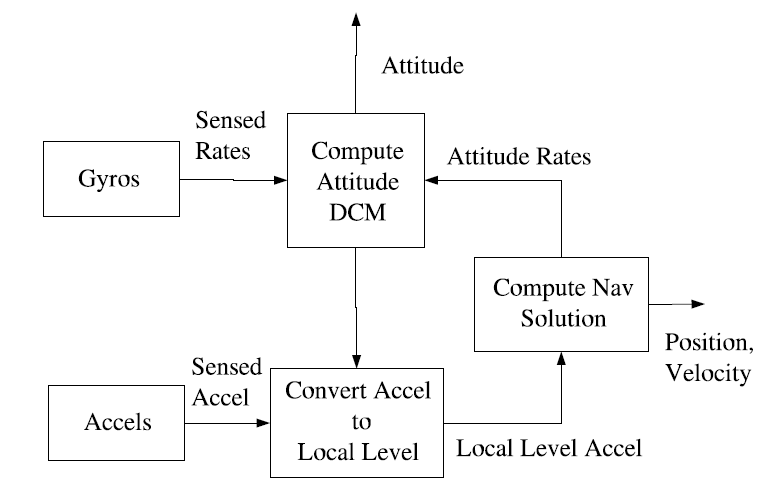
\includegraphics[scale=0.5]{graphics/strapdown_block.png}
\end{center}
\end{frame}

\begin{frame}
\frametitle{Basic Strapdown Navigation Equations}
 \begin{itemize}
 \item Need to compute attitude, velocity, and position
 \item I.e., need to compute $\dcm{B}{L}$ and $\dcm{L}{E}$
 \item These DCMs are dynamic quantities
 \item $\dcm{B}{L}$ determines attitude and can be rapidly varying
 \item $\dcm{L}{E}$ determines position and is slowly varying (relative to attitude dynamics)
\end{itemize}
\end{frame}


\begin{frame}
\frametitle{Strapdown Navigation Equations}
 \begin{itemize}
 \item Three differential equations
 \begin{itemize}
   \item Equation for body to local level transformation $\dcm{B}{L}$
   \item Equation for velocity (uses $\dcm{B}{L}$)
   \item Equation for local level to earth for position DCM $\dcm{L}{E}$
 \end{itemize}
\end{itemize}
\end{frame}

\begin{frame}
Strapdown Navigation Equations
 \begin{itemize}
 \item Two Algebraic Equations
 \begin{itemize}
   \item Equation for converting velocity to transport rate (to be explained)
   \item Equation for converting earth rate to local level
   coordinates
 \end{itemize}
\end{itemize}
\end{frame}
\begin{frame}
\frametitle{Strapdown Navigation Equations}
\framesubtitle{The Three Differential Equations}
\begin{equation}\label{cbleq}
  \cbleq
\end{equation}
\begin{equation}\label{strapveleq}
  \strapveleq
\end{equation}
\begin{equation}\label{cleeq}
  \cleeq
\end{equation}
\end{frame}

\begin{frame}
\frametitle{Strapdown Navigation Equations}
\framesubtitle{The Two Algebraic Equations}
\begin{equation}\label{trateeq}
  \trateeq \text{ (wander azimuth $\rho_z=0$)}
\end{equation}
\begin{equation}\label{erateeq}
  \erateeq
\end{equation}
\end{frame}

\begin{frame}
\frametitle{Strapdown Navigation Equations}
The $\dcm{B}{L}$ Equation \eqref{cbleq}
\[\cbleq\]
\begin{itemize}
\item All the $\Omega$ matrices represent rotation vector cross products in skew-symmetric matrix format
\begin{itemize}
 \item $\rotmat{I}{B}^B$ is rotational rate of aircraft in body
coordinates
\item $\rotmat{I}{E}^L$ is earth rate in local level coordinates
\item $\rotmat{E}{L}^L$ is transport rate in local level
coordinates
\end{itemize}
\end{itemize}
\end{frame}

\begin{frame}
\frametitle{Strapdown Navigation Equations: Detour into Cross Product Matrices}
\begin{itemize}
\item The cross product of $\omega=\colvecthree{\omega}{}$ with any other vector $v$ is the same as multiplying $v$ on the left by
$\Omega = \skewsymmat{\omega}{1}{2}{3}$
\item $\omega \times v=\Omega v$
\end{itemize}
\end{frame}

\begin{frame}
\frametitle{Strapdown Navigation Equations}
The $\dcm{B}{L}$ Equation \eqref{cbleq}
\[\cbleq\]
\begin{itemize}
\item Transport rate is the rotational rate of the aircraft due to
motion over the surface of the earth.  Is a function of velocity.
\item $\rotmat{I}{B}^B$ is total inertial angular rate sensed by gyros and includes effects of
transport and earth rates.
\item Hence transport and earth rate effects have to be subtracted
off.
\end{itemize}
\end{frame}

\begin{frame}
\frametitle{Strapdown Navigation Equations}
\framesubtitle{The Strapdown Velocity Equation} \eqref{strapveleq}
\[\strapveleq\]
 \begin{itemize}
 \item Sometimes referred to as the velocity rate equation
 \item $\specforce^B$ is specific force sensed by accelerometers in
 body coordinates (because the accels are strapped to the body --
 hence the term strapdown)
\end{itemize}
\end{frame}

%\begin{frame}
%\includegraphics[width=10in,height=6.5in]{strapnav_block.png}
%\end{frame}

\begin{frame}
\frametitle{Strapdown Navigation Equations}
\framesubtitle{The Transport Rate Equation}
 \eqref{cleeq}
\[\cleeq\]
\begin{itemize}
  \item Connected to velocity rate equation by the first algebraic equation \eqref{trateeq}:
\[\trateeq\]
  \item Eq. \eqref{cleeq} Sometimes referred to as position rate equation, because $\dcm{L}{E}$ directly implies the vehicle position
\end{itemize} 
\end{frame}

\begin{frame}
\frametitle{Strapdown Navigation Equations}
\framesubtitle{Position Rate / Transport Rate Equations (Geographic)}
\begin{itemize}
  \item North transport rate:
\begin{equation}\label{trateneq}
\trateneq
\end{equation} 
  \item East transport rate:
\begin{equation}\label{trateeeq}
\trateeeq
\end{equation} 
where $e$ is ellipticity (approx. $\dfrac{1}{298}$) and $R_e$ is mean equatorial earth radius
\end{itemize} 
\end{frame}

\begin{frame}
\frametitle{Strapdown Navigation Equations}
\framesubtitle{Position Rate / Transport Rate Equations (Geographic)}
\begin{itemize}
  \item Latitude Rate:
\begin{equation}\label{latrate}
\latrateeq
\end{equation}  
  \item Longitude Rate:
\begin{equation}\label{lonrate}
\lonrateeq
\end{equation}  
\end{itemize} 
\end{frame}

\begin{frame}
\frametitle{Strapdown Navigation Equations}
\begin{itemize}
  \item Geographic (north-slaved) mechanization has singularities at poles
  \item Two other approaches to local level coordinates:
  \begin{itemize}
	\item Free azimuth: vertical component of transport rate $\rho_z$= additive inverse of vertical component of earth rate
	\item Wander Azimuth:  vertical component of transport rate $\rho_z$ = 0
  \end{itemize}
\end{itemize} 
\end{frame}

\begin{frame}
\frametitle{Strapdown Navigation Equations}
\framesubtitle{Position Rate / Transport Rate Equations (Wander and Free Azimuth)}
\begin{itemize}
  \item X Transport Rate:
\begin{align}\label{xtrateeq}
\xtrateeq
\end{align}  
  \item Y Transport Rate:
\begin{align}\label{ytrateeq}
\ytrateeq
\end{align}  
\end{itemize} 
\end{frame}

\begin{frame}
\frametitle{Strapdown Navigation Equations}
\framesubtitle{Position Rate / Transport Rate Equations (Wander and Free Azimuth)}
\begin{itemize}
  \item Azimuth Rate:
\[
\rho_z= 
\begin{cases} 
-\erate d_{23}, &\text{if free azimuth;}\\ 
0,  &\text{if wander azimuth} 
\end{cases}
\]
  \item In equations above, the matrix $\left[d_{ij}\right]$ is the direction cosine matrix $\dcm{L}{E}$ from local level (L) frame to earth centered earth fixed (E) frame.
\end{itemize} 
\end{frame}


\begin{frame}
\frametitle{GPS}
\begin{itemize}
  \item Trilateration:  Knowing the distance from an unknown point to three known points yields the coordinates of the unknown point
  \item What if the distances are not known precisely?  
Answer:  Use 'pseudorange' instead, i.e., use signals traveling at speed of light and very accurate clocks
  \item What if the coordinates of the three points are not really known precisely?  Answer:  Use your best guess!
\end{itemize} 
\end{frame}

\begin{frame}
	\frametitle{Trilateration}
	\begin{figure}
	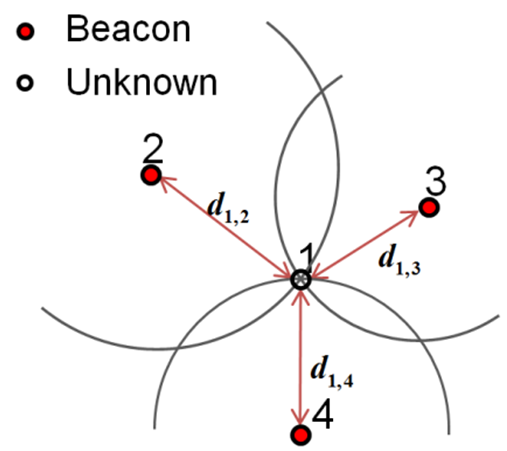
\includegraphics[width=0.5\textwidth]{graphics/trilateration.png}
\caption{Trilateration:  Distances to Three Beacons}
	\end{figure}
\end{frame}


\begin{frame}
	\frametitle{Pseudorange}
	\begin{itemize}
		\item distance = (speed of signal) $\times$ (time of signal flight)
		\begin{itemize}
			\item $\rho = c\Delta t$
		\end{itemize}
		\item Called 'pseudorange' because it is not a true range; it is only apparent due to inaccurate clocks
		\item By the same token, the coordinates of the transmitting satellites are also not known precisely, and so we could speak of 'pseudopositions' as well.   But nobody does that!
	\end{itemize}
\end{frame}

\begin{frame}
	\frametitle{Satellite Position}
	\begin{itemize}
		\item How do we know which satellite is transmitting? Answer:  Unique Pseudorandom Noise (PRN)
		\item How we know the position of the 
satellite at time of transmission?  Answer:
		\begin{itemize}
			\item Six Keplerian elements
			\item User receiver converts to WGS-84 X,Y,Z ECEF coordinates
		\end{itemize}
	\end{itemize}
\end{frame}

\begin{frame}
	\frametitle{Six Keplerian Elements}
	\begin{itemize}
		\item Eccentricity
		\item Semi-major axis
		\item Inclination
		\item Longitude of the ascending node
		\item Argument of periaspsis
		\item Mean anomaly
	\end{itemize}
\end{frame}

\begin{frame}
\frametitle{Keplerian Elements}
	\begin{figure}
	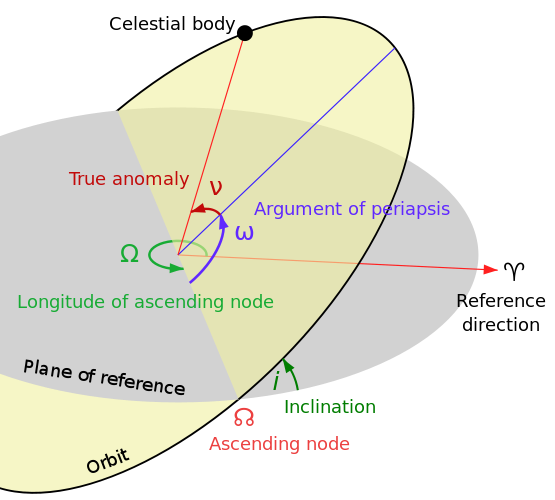
\includegraphics[width=0.75\textwidth,height=0.75\textheight]{graphics/555px-Orbit1_svg.png}
%	\caption{Keplerian Elements}
	\end{figure}
\end{frame}

\begin{frame}
\frametitle{Keplerian Elements}
	\begin{figure}
	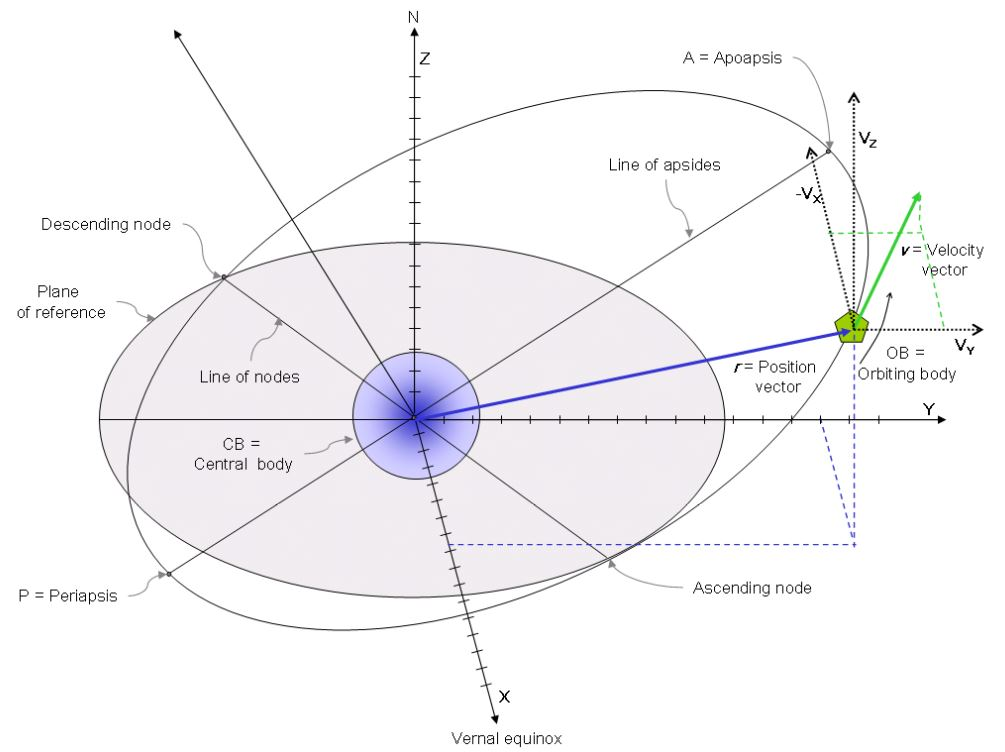
\includegraphics[width=0.80\textwidth,height=0.80\textheight]{graphics/keplerian_elements2.jpg}
%	\caption{Keplerian Elements}
	\end{figure}
\end{frame}

\begin{frame}
\frametitle{IS-GPS-200 Table 20-II}
\framesubtitle{1 of 2}
	\begin{figure}[h]
	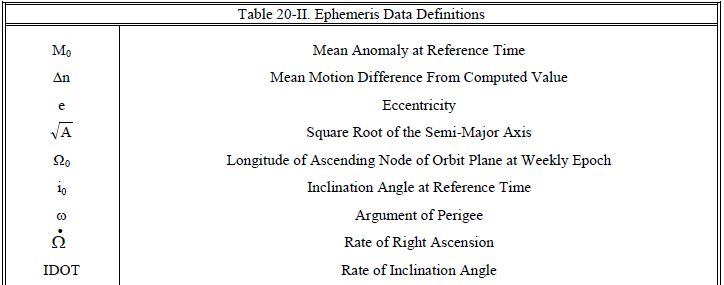
\includegraphics[width=0.8\textwidth]{graphics/table20-II-A.jpg}
%	\caption{Keplerian Elements}
	\end{figure}
\end{frame}

\begin{frame}
\frametitle{IS-GPS-200 Table 20-II}
\framesubtitle{2 of 2}
	\begin{figure}[h]
	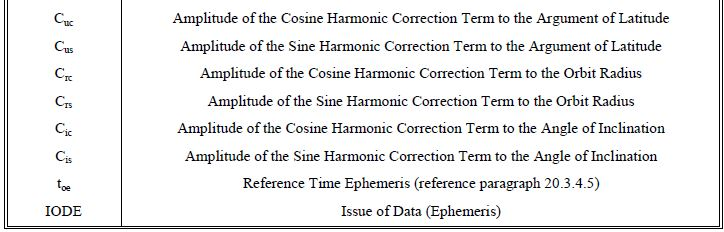
\includegraphics[width=0.8\textwidth]{graphics/table20-II-B.jpg}
%	\caption{Keplerian Elements}
	\end{figure}
\end{frame}

\begin{frame}
\frametitle{IS-GPS-200 Table 20-IV}
\framesubtitle{Elements of Coordinate Systems (1 of 3)}
	\begin{figure}[h]
	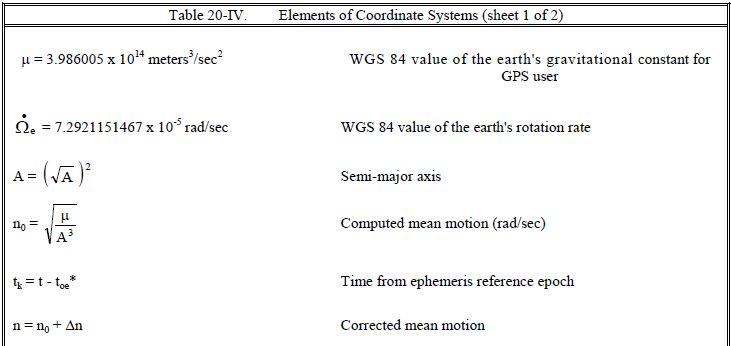
\includegraphics[width=0.8\textwidth]{graphics/table20-IV-A.jpg}
%	\caption{Keplerian Elements}
	\end{figure}
\end{frame}

\begin{frame}
\frametitle{IS-GPS-200 Table 20-IV}
\framesubtitle{Elements of Coordinate Systems (2 of 3)}
	\begin{figure}[h]
	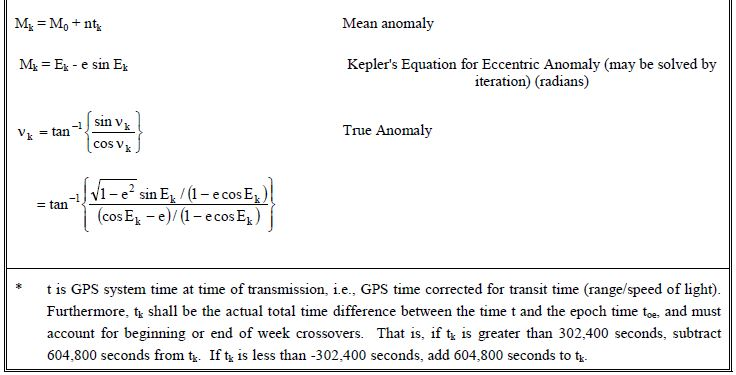
\includegraphics[width=0.8\textwidth]{graphics/table20-IV-B.jpg}
%	\caption{Keplerian Elements}
	\end{figure}
\end{frame}

\begin{frame}
\frametitle{IS-GPS-200 Table 20-IV}
\framesubtitle{Elements of Coordinate Systems (3 of 3)}
	\begin{figure}[h]
	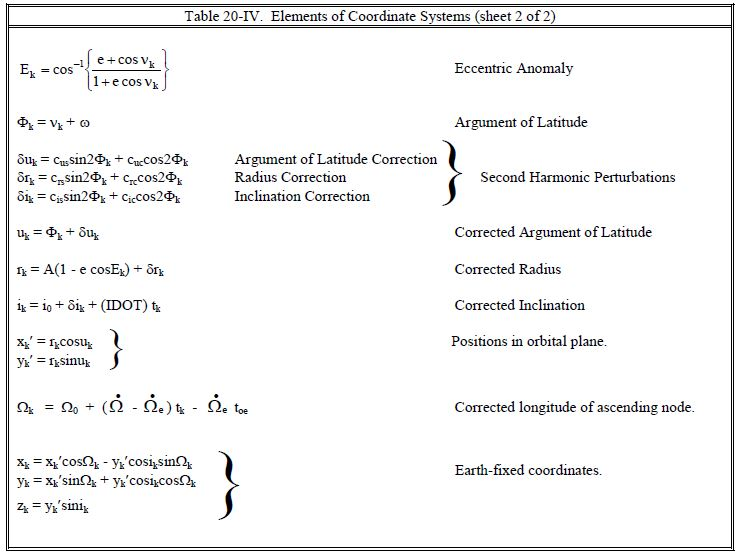
\includegraphics[width=0.8\textwidth]{graphics/table20-IV-C.jpg}
%	\caption{Keplerian Elements}
	\end{figure}
\end{frame}


% day3_seg2_inertial/inertial_main.tex
\begin{frame}
  \onslide<1->{
	\frametitle{Inertial Error Dynamics} 
	\framesubtitle{Topics}
}
\begin{itemize}
  \onslide<2->{
 \item Imperfect Inertial Instruments
}
  \onslide<3->{
 \item From Strapdown Equations to Error Equations
}
  \onslide<4->{
 \item Initialization: Alignment
}
\end{itemize}
\end{frame}
% day3_seg2_inertial/impinst.tex
\begin{frame}
  \onslide<1->{
	\frametitle{Inertial Error Dynamics} 
	\framesubtitle{Imperfect Inertial Instruments}
}
\begin{itemize}
  \onslide<2->{
 \item Accelerometers and Gyros have inherent imperfections
}
  \onslide<3->{
 \item Bias, scale factor, $g^2$ terms, noise, random walks, etc.
}
  \onslide<4->{
 \item Inertial sensor clusters also have errors: misalignments
}
  \onslide<5->{
 \item Many error sources are calibrated out using rate tables during ATP
}
 \onslide<6->{ 
 \item Residual effects will influence strapdown nav equations
}
\end{itemize}
\end{frame}

\begin{frame}
  \onslide<1->{
	\frametitle{Inertial Error Dynamics} 
	\framesubtitle{Imperfect Inertial Instruments}
}
\begin{itemize}
  \onslide<2->{
  \item Strapdown nav equations very sensitive to gyro errors
}
  \onslide<3->{
  \item Gyro biases yield erroneous $\dcm{B}{L}$ matrix which in turn causes erroneous accelerations to be computed in local level frame
}
  \onslide<4->{
  \item Thus, gyro errors affect not only attitude, but also position and velocity
}
\end{itemize}
\end{frame}

\begin{frame}
  \onslide<1->{
	\frametitle{Inertial Error Dynamics} 
	\framesubtitle{Simple Inertial Error Models}
}
\begin{itemize}
  \onslide<2->{
  \item Gyros
\[
\simprateerreq{x}{y}{z}
\]
\[
\simprateerreq{y}{z}{x}
\]
\[
\simprateerreq{z}{x}{y}
\]

where $\gyrobias{i}$ is the $i^\text{th}$ gyro bias, $\gyrosf{i}$ the $i^\text{th}$ gyro scale factor, and $\gyromisalign{i}{j}$ is the misalignment of the $i^\text{th}$ gyro axis toward the $j^\text{th}$ gyro axis. 
}
\end{itemize}
\end{frame}

\begin{frame}
  \onslide<1->{
	\frametitle{Inertial Error Dynamics} 
	\framesubtitle{Simple Inertial Error Models}
}
\begin{itemize}
  \onslide<2->{
  \item Accelerometers
\[
\simpaccelerreq{x}{y}{z}
\]
\[
\simpaccelerreq{y}{z}{x}
\]
\[
\simpaccelerreq{z}{x}{y}
\]
where $\accelbias{i}$ is the $i^\text{th}$ accelerometer bias, $\accelsf{i}$ the $i^\text{th}$ accelerometer scale factor, and $\accelmisalign{i}{j}$ is the misalignment of the $i^\text{th}$ accelerometer axis toward the $j^\text{th}$ accelerometer axis. 
}
\end{itemize}
\end{frame}


\begin{frame}
  \onslide<1->{
	\frametitle{Inertial Error Dynamics} 
	\framesubtitle{Bias Models}
}
\begin{itemize}
  \onslide<2->{
  \item Bias in both types of instruments can be further broken down into several components:
  \begin{itemize}
	\item fixed bias -- constant from turn-on to turn-on -- should be calibrated out
	\item bias stability -- varies from turn-on to turn-on -- can't be calibrated out, but can be characterized in terms of variance -- can model as random constant
	\item bias drift -- usually modeled as random walk
  \end{itemize} 
}
\end{itemize}
\end{frame}


\begin{frame}
  \onslide<1->{
	\frametitle{Inertial Error Dynamics} 
	\framesubtitle{Scale Factor Models}
}
\begin{itemize}
  \onslide<2->{
  \item Scale factor can also be modeled as a sum of three components
}
  \onslide<3->{
  \item Often in nav filters, scale factor residual is modeled as a random constant
}
  \onslide<4->{
  \item Important to keep in mind that the contribution of scale factor error is a function of input (rate or acceleration) 
}
\end{itemize}
\end{frame}
\begin{frame}
  \onslide<1->{
	\frametitle{Inertial Error Dynamics} 
	\framesubtitle{Higher Order Models}
}
\begin{itemize}
  \onslide<2->{
  \item In expanding the output error as a Taylor series function of input, bias, scale factor, and misalignment show up as zero and first order terms.
}
  \onslide<3->{
  \item Higher order terms are also present, especially second order terms.
}
  \onslide<4->{
  \item In some calibration and alignment filters, such higher order effects are modelled
}
  \onslide<5->{
  \item SNU-84-1 includes error budgets associated with all the combined, higher order effects.  
}
\end{itemize}
\end{frame}

\begin{frame}
  \onslide<1->{
	\frametitle{Inertial Error Dynamics} 
	\framesubtitle{Higher Order Models:  Taylor Series of Two Variables}
}
  \onslide<2->{
\begin{align*}
\gentaylordouble{f}{x}{y}{x_0}{y_0}
\end{align*}
Taylor Series provides basis for all error analysis.
}
\end{frame}

\subsection{Strapdown Error Dynamics}
% day3_seg2_inertial/straperr.tex
\begin{frame}
  \onslide<1->{
	\frametitle{Inertial Error Dynamics} 
	\framesubtitle{From Strapdown Equations to Error Equations}
}
\begin{itemize}
  \onslide<2->{
 \item Nav equations require perfect inertial instruments
}
  \onslide<3->{
 \item Instruments are not perfect
}
  \onslide<4->{
 \item Inertial instrument error sources (bias, scale factor errors, etc.) generate erroneous rate and acceleration inputs to the nav equations  
}
  \onslide<5->{
 \item Need to figure out the effects on the outputs of these equations
}
\end{itemize}
\end{frame}
% cm_kf_talk_straperr.tex


\begin{frame}
  \onslide<1->{
	\frametitle{Inertial Error Dynamics} 
	\framesubtitle{Strapdown Error Equations}
}
\begin{itemize}
  \onslide<2->{
 \item Nature of Errors
}
  \onslide<3->{
 \item Error Operator
}
  \onslide<4->{
 \item Error Equations
}
\end{itemize}
\end{frame}


\begin{frame}
  \onslide<1->{
	\frametitle{Inertial Error Dynamics} 
	\framesubtitle{Strapdown Error Equations: Nature of Errors}
}
\begin{itemize}
  \onslide<2->{
 \item Errors propagate according to derived equations
}
  \onslide<3->{
 \item Errors are generally small, so approximating assumptions
 help simplify the math
 \begin{itemize}
}
  \onslide<4->{
 \item linearize otherwise non-linear dynamics
}
  \onslide<5->{
 \item small angle assumptions:  $\sin\theta \approx \theta$
 \end{itemize}
}
\end{itemize}
\end{frame}


\begin{frame}
  \onslide<1->{
	\frametitle{Inertial Error Dynamics} 
	\framesubtitle{Strapdown Error Equations: Error Operator}
}
\begin{itemize}
  \onslide<2->{
\item   If $A$ is any quantity, we define error operator as follows:
\begin{equation}\label{errop}
  \errop{A},
\end{equation}
where $A$ is the true quantity of interest and $\hat{A}$ is an
apparent quantity.  The latter could be a measured value, and
estimated value, or some computed value.  This means that
\[\hat{A}=A+\delta A\]
i.e., the apparent value is the true value plus some error.

}
\end{itemize}
\end{frame}


\begin{frame}
  \onslide<1->{
	\frametitle{Inertial Error Dynamics} 
	\framesubtitle{Strapdown Error Equations: Error Operator}
}
\begin{itemize}
  \onslide<2->{
\item   Error operator satisfies:
\begin{equation}\label{erropid}
  \delta(AB) = \delta A \cdot B + A \cdot \delta B
\end{equation}
}
  \onslide<3->{
\item   Proof:
\begin{align*}
\delta(AB) &= \widehat{AB} - AB\\
&= \hat{A}\hat{B}-AB\\
&= (A+\delta A)(B+\delta B)-AB\\
&= AB + A\cdot\delta B +\delta A \cdot B + \delta A \cdot \delta B - AB\\
& = \delta A \cdot B + A\cdot\delta B
\end{align*}
since we may assume that $\delta A \cdot\delta B \approx 0$.
}
\end{itemize}
\end{frame}


\begin{frame}
  \onslide<1->{
	\frametitle{Inertial Error Dynamics} 
	\framesubtitle{Strapdown Error Equations}
}
\begin{itemize}
  \onslide<2->{
\item   Applying these to the three differential equations, yields three
error equations:
\begin{equation}\label{cblerreq}
  \cblerreq
\end{equation}
\begin{equation}\label{strapvelerreq}
  \strapvelerreq
\end{equation}
\begin{equation}\label{cleerreq}
  \cleerreq
\end{equation}
}
\end{itemize}
\end{frame}



\begin{frame}
  \onslide<1->{
	\frametitle{Inertial Error Dynamics} 
	\framesubtitle{Strapdown Error Equations}
}
\begin{itemize}
  \onslide<2->{
\item   Introducing \textbf{small angular rotations} for tilt and position
\begin{itemize}
}
  \onslide<3->{
  \item $\compdcm{B}{L}$, the computed (i.e., apparent) version of $\dcm{B}{L}$ is related additively to the true version by the error $\delta \dcm{B}{L}$
\[\compdcm{B}{L}= \dcm{B}{L}+ \delta \dcm{B}{L}\]
}
  \onslide<4->{
  \item It is also related to $\dcm{B}{L}$ by a small direction cosine matrix relating the local level frame to the computer frame $\widehat{L}$:
\[\compdcm{B}{L}= \dcm{L}{\widehat{L}}\dcm{B}{L}\] 
\end{itemize} 
}
\end{itemize}
\end{frame}

\begin{frame}
  \onslide<1->{
	\frametitle{Inertial Error Dynamics} 
	\framesubtitle{Strapdown Error Equations}
}
\begin{itemize}
  \onslide<2->{
\item Substituting the second equation into the first allows us to solve for $\delta \dcm{B}{L}$:
\begin{align*}
\delta \dcm{B}{L} &= \compdcm{B}{L} -\dcm{B}{L}\\
&= \dcm{L}{\widehat{L}}\dcm{B}{L}-\dcm{B}{L}\\
&= (\dcm{L}{\widehat{L}} - I)\dcm{B}{L}
\end{align*}
Now, let's introduce $\Phi=I-\dcm{L}{\widehat{L}}$ to obtain:
\[\delta \dcm{B}{L}=-\Phi\dcm{B}{L}\]
}
\end{itemize}
\end{frame}


\begin{frame}
  \onslide<1->{
	\frametitle{Inertial Error Dynamics} 
	\framesubtitle{Strapdown Error Equations}
}
\begin{itemize}
  \onslide<2->{
  \item Using small angle approximations, $\dcm{L}{\widehat{L}}$ can be written in the form
\[\dcm{L}{\widehat{L}}=
\begin{bmatrix}
1&\phi_z&-\phi_y\\
-\phi_z&1&\phi_x\\
\phi_y&-\phi_x&1
\end{bmatrix}.
\]
Thus, $\Phi=I-\dcm{L}{\widehat{L}}$ is seen to be a skew-symmetric rotation matrix:
\[\Phi=
\begin{bmatrix}
0&-\phi_z&\phi_y\\
\phi_z&0&-\phi_x\\
-\phi_y&\phi_x&0
\end{bmatrix}.
\]
}
\end{itemize}
\end{frame}


\begin{frame}
  \onslide<1->{
	\frametitle{Inertial Error Dynamics} 
	\framesubtitle{Strapdown Error Equations}
}
\begin{itemize}
  \onslide<2->{
  \item $\Phi$ is therefore equal to the cross product operator associated with a vector $\phi^L = \begin{bmatrix}\tiltx^L & \tilty^L & \az^L \end{bmatrix}\trans$.  I.e.,
\[\Phi = \xop{\phi^L}\]
}
  \onslide<3->{
\item The three components of $\phi^L$ will become three states in our inertial error dynamics Kalman filter.
}
  \onslide<4->{
\item $\phi_x$ and $\phi_y$ are called tilts, while $\psi_z$ is called the azimuth error.
}
\end{itemize}
\end{frame}


\begin{frame}
  \onslide<1->{
	\frametitle{Inertial Error Dynamics} 
	\framesubtitle{Strapdown Error Equations}
}
\begin{itemize}
  \onslide<2->{
  \item By a similar derivation, we can introduce a small angular position angle error $e^L=\begin{bmatrix}e_x^L & e_y^L & e_z^L \end{bmatrix}\trans$
}
  \onslide<3->{
  \item $e^L$ is associated with $\delta\dcm{E}{L}$ just as $\phi^L$ is associated with $\delta\dcm{B}{L}$:
\[\delta\dcm{E}{L}=-E^L\dcm{E}{L},\]
where $E^L$ is the skew-symmetric matrix form of $e^L$.
}
  \onslide<4->{
  \item The three components of $e^L$ yield the three position error states in a typical navigation Kalman filter.
}
\end{itemize}
\end{frame}


\begin{frame}
  \onslide<1->{
	\frametitle{Inertial Error Dynamics} 
	\framesubtitle{Strapdown Error Equations}
}
\begin{itemize}
  \onslide<2->{
  \item We are working to simplify Eq. \eqref{cblerreq}:
\[\cblerreq\]
}
  \onslide<3->{
  \item We have an expression for $\delta \dcm{B}{L}$.
}
\end{itemize}
\end{frame}


\begin{frame}
  \onslide<1->{
	\frametitle{Inertial Error Dynamics} 
	\framesubtitle{Strapdown Error Equations}
}
\begin{itemize}
  \onslide<2->{
  \item Consider the earth rate error term $\delta \rotmat{I}{E}^L$.  Since $\rotmat{I}{E}^L=\dcm{E}{L}\rotmat{I}{E}^E$ and $\delta\rotmat{I}{E}^E=0$, we derive:
\[\delta\rotmat{I}{E}^L=\delta\dcm{E}{L}\rotmat{I}{E}^E.\]
}
  \onslide<3->{
  \item But $\delta\dcm{E}{L}=-E^L\dcm{E}{L}$.  Therefore,
\begin{align*}
\delta\rotmat{I}{E}^L&=-E^L\dcm{E}{L}\rotmat{I}{E}^E\\
&=-E^L\rotmat{I}{E}^L.
\end{align*}
}
\end{itemize}
\end{frame}


\begin{frame}
  \onslide<1->{
	\frametitle{Inertial Error Dynamics} 
	\framesubtitle{Strapdown Error Equations}
}
\begin{itemize}
  \onslide<2->{
  \item For the error in transport rate, $\delta\rotmat{E}{L}^L$, using the error operator on Eq. \eqref{trateeq}, a new error terms having to do with altitude error shows up:
\begin{align*}
\delta\rotvec{E}{L}^L&=\delta\left[\dfrac{1}{R}u_r^L\times v^L\right]\\
&=\dfrac{1}{R}u_r^L\times \delta v^L - \dfrac{\delta h}{R^2}\left[u_r^L\times v^L\right]
\end{align*}
}
  \onslide<3->{
\item Here, $R=R_e+h$ for a spherical earth of radius $R_e$.
}
\end{itemize}
\end{frame}


\begin{frame}
  \onslide<1->{
	\frametitle{Inertial Error Dynamics} 
	\framesubtitle{}
}
\begin{itemize}
  \onslide<2->{
  \item Eq. \eqref{cblerreq} can now be rewritten as:
\begin{equation}\label{tilteq}
\tilteq
\end{equation} 
where $\delta \rotmat{E}{L}^L$ is the skew-symmetric matrix form of 
\[\trateerreqsphere\]
}
\end{itemize}
\end{frame}


\begin{frame}
  \onslide<1->{
	\frametitle{Inertial Error Dynamics} 
	\framesubtitle{Strapdown Error Equations}
}
\begin{itemize}
  \onslide<2->{
  \item Similarly, the velocity equation can be rewritten:
\begin{align*}
\velerreq
\end{align*} 
while the equation for the position angle error $e^L$ itself is
\begin{equation}
\paeeq
\end{equation} 
}
\end{itemize}
\end{frame}




\begin{frame}
  \onslide<1->{
	\frametitle{Inertial Error Dynamics} 
	\framesubtitle{Strapdown Error Equations}
}
\begin{itemize}
  \onslide<2->{
\item   Further Simplifications Using Telescope Pointing Angle Error

}
  \onslide<3->{
  \item $\psi^L = \phi^L - e^L$
}
  \onslide<4->{
  \item Leads to:
}
  \onslide<5->{
\begin{equation}\label{deltardoteq}
\deltardoteq
\end{equation}
and
\begin{eqnarray}
\velerreqpsi
\end{eqnarray}  
}
\end{itemize}
\end{frame}



\begin{frame}
  \onslide<1->{
	\frametitle{Inertial Error Dynamics} 
	\framesubtitle{Strapdown Error Equations}
}
\begin{itemize}
  \onslide<2->{
  \item Finally, the equations for the telescope pointing angle errors are: 
}
  \onslide<3->{
\begin{equation}\label{telscopeeq}
\telscopeeq
\end{equation}
}
\end{itemize}
\end{frame}

\begin{frame}
  \onslide<1->{
	\frametitle{Inertial Error Dynamics} 
	\framesubtitle{Strapdown Error Equations}
}
\begin{itemize}
  \onslide<2->{
 \item Three error equations yield three vector quantities of
 interest
 \begin{itemize}
}
  \onslide<3->{
 \item position error vector (3) $\poserr$ derived from $\delta \dcm{L}{E}$
}
  \onslide<4->{
 \item velocity error vector (3) $\velerr^L$ (or $\delta v^L$)
}
  \onslide<5->{
 \item attitude error vector (3) $\tiltx,\tilty,\az$ from $\delta \dcm{B}{L}$
 \end{itemize}
}
\end{itemize}
\end{frame}

\begin{frame}
  \onslide<1->{
	\frametitle{Inertial Error Dynamics} 
	\framesubtitle{Strapdown Error Equations}
}
\begin{itemize}
  \onslide<2->{
  \item See Matlab / Simulink Models
	\begin{itemize}
}
  \onslide<3->{
	  \item Strapdown Navigation Equations: TBD
}
  \onslide<4->{
	  \item Strapdown Navigation Error Equations: TBD
    \end{itemize}
}
\end{itemize}
\end{frame}


\subsection{Inertial Alignment}
% day3_seg2_inertial/align.tex
\begin{frame}
Initialization:  Alignment
 \begin{itemize}
 \item Coarse Leveling
  \begin{itemize}
    \item Gimbal system limited by platform torquing rates
    \item Strapdown systems have no real rate limits
    \item Time average of accel outputs scaled by $1/g$
	\item Yields third row of DCM to begin fine alignment
  \end{itemize}
 \item Fine Alignment
 \item Alignment filter aids in further leveling
\end{itemize}
\end{frame}

%% day3_seg2_inertial/exercises.tex
\begin{frame}
Exercises
 \begin{itemize}
 \item
 \item
 \item
\end{itemize}
\end{frame}


% day3_seg3_9-state/9-state_main.tex
\begin{frame}
  \onslide<1->{
	\frametitle{The Basic 9-State Kalman Filter} 
	\framesubtitle{Topics}
}
\begin{itemize}
  \onslide<2->{
 \item Whole State Filters vs. Error State Filters
}
  \onslide<3->{
 \item The Canonical Nine States
}
  \onslide<4->{
 \item INS Error State Dynamics and Transition Matrix
}
\end{itemize}
\end{frame}
% day3_seg3_9-state/whole_error.tex
\begin{frame}
  \onslide<1->{
	\frametitle{9-state Filter} 
	\framesubtitle{Whole State vs. Error State Filters}
}
\begin{itemize}
  \onslide<2->{
 \item Whole state filters ...
}
  \onslide<3->{
 \begin{itemize}
 \item model whole position, velocity, attitude
}
  \onslide<4->{
 \item deal with large and rapidly varying quantities
}
  \onslide<5->{
 \item are highly non-linear
 \end{itemize}
}
\end{itemize}
\end{frame}


\begin{frame}
  \onslide<1->{
	\frametitle{9-state Filter} 
	\framesubtitle{Whole State vs. Error State Filters}
}
\begin{itemize}
  \onslide<2->{
  \item Error state filters ...
}
  \onslide<3->{
	\begin{itemize}
	  \item remove some of the nonlinearities by differencing outputs from aiding sensors with corresponding quantities from INS
}
  \onslide<4->{
	  \item exhibit slowly varying dynamics:  easier to linearize
}
  \onslide<5->{
	  \item have smaller quantities that allow us to take advantage of small angle assmptions
	\end{itemize}
}
\end{itemize}
\end{frame}

% day3_seg3_9-state/9states.tex
\begin{frame}
  \onslide<1->{
	\frametitle{The Canonical Nine States} 
	\framesubtitle{}
}
\begin{itemize}
  \onslide<2->{
 \item 3 position errors: $\poserr_x,\poserr_y,\poserr_z$ in local level coordinates
}
  \onslide<3->{
 \item 3 velocity errors: $\velerr_x,\velerr_y,\velerr_z$ in local level coordinates
}
  \onslide<4->{
 \item 3 attitude errors: $\tiltx,\tilty,\az$
}
  \onslide<5->{
	\begin{itemize}
	  \item $\tiltx,\tilty$ known as tilt errors
	  \item $\az$ known as azimuth error
	\end{itemize}
}
\end{itemize}
\end{frame}

%\input{day3_seg3_9-state/inserrdyn.tex}
% day3_seg3_9-state/exercises.tex
\begin{frame}
  \onslide<1->{
	\frametitle{Exercises} 
	\framesubtitle{}
}
\begin{itemize}
  \onslide<2->{
\item   1. Rewrite equation \eqref{cblerreq}
\[\cblerreq\]
to show the terms in the canonical order with position error, velocity error, and then attitude error.

}
  \onslide<3->{
\item   2. Determine the $7^\text{th}$ row of the system matrix $F$ for the canonical 9-state error model.  Use the cross-product operator 
matrix as required, e.g.,
$\rotmat{I}{E}^L=\xop{\omega_{IE}^L}=\xopdef{\left[\omega_{IE}^L\right]}$.  Introduce simplifying notation!  
E.g., set $\alpha=\omega_{IE}^L$  Hint:  Use telescope pointint angle error equation \eqref{telscopeeq}

}
\end{itemize}
\end{frame}

%% 15states.tex
\begin{frame}
A 15-State Inertial Error Model: State Vector
\[x=\fsvec\]
\end{frame}

\begin{frame}
\footnotesize 
\setlength{\arraycolsep}{2.5pt} 
\medmuskip = 1mu % default: 4mu plus 2mu minus 4mu
A 15-State Inertial Error Model: State Dynamics Matrix
\[\fssdm\]
where $T$ is the delta time interval, $\tau_g$,$\tau_a$,$\tau_N$,$\tau_E$ are Markov time corelation constants 
for gyro bias, accelerometer bias and GPS north and east biases, respectively. 
\end{frame}




% day3_seg4_ins_challenges/ins_chal_main.tex
\begin{frame}
  \onslide<1->{
	\frametitle{Challenges of INS Filters} 
	\framesubtitle{}
}
\begin{itemize}
  \onslide<2->{
 \item Nine States Are Not Enough
}
  \onslide<3->{
 \item Not Constant Coefficient
}
  \onslide<4->{
 \item Non-Linearities: Extended Kalman Filter
}
  \onslide<5->{
 \item Observability
}
\end{itemize}
\end{frame}
%day3_seg4_ins_challenges/9notenough.tex
\begin{frame}
  \onslide<1->{
	\frametitle{Nine States Are Not Enough} 
	\framesubtitle{}
}
\begin{itemize}
  \onslide<2->{
 \item The canoncial 9 states only characterize the inertial error dynamics
}
  \onslide<3->{
 \item They treat of the inner coupling between inertial error sources
}
  \onslide<4->{
 \item However, they don't help characterize dynamics of aiding sensor errors
}
  \onslide<5->{
  \item They don't help estimate aiding states such as Doppler bias and boresight errors
}
  \onslide<6->{
  \item Or GPS receiver clock errors
  }
  \onslide<7->{  
  \item They also don't help us to estimate inertial instrument drifts such as bias drift or scale factor errors
}
\end{itemize}
\end{frame}

%day3_seg4_ins_challenges/notconstcoeff.tex
\begin{frame}
  \onslide<1->{
	\frametitle{Not Constant Coefficient} 
	\framesubtitle{}
}
\begin{itemize}
  \onslide<2->{
 \item Notice that the $F$ matrix that has emerged (implicitly) from the 9-state inertial error dynamics is not time invariant
}
  \onslide<3->{
 \item It is highly dependent on trajectory data such as acceleration and angular rate profiles
}
  \onslide<4->{
 \item These are functions of time
}
  \onslide<5->{
 \item Position dependent items such as latitude are also involved
}
\end{itemize}
\end{frame}

% day3_seg4_ins_challenges/nonlinear.tex
\begin{frame}
  \onslide<1->{
	\frametitle{Non-Linearities: Extended Kalman Filter} 
	\framesubtitle{}
}
\begin{itemize}
  \onslide<2->{
 \item When non-linearities are present, the $F$ matrix emerges as Jacobian of non-linear system function $f$:  $F(t)=\dfrac{\partial f}{\partial x}$
}
  \onslide<3->{
  \item If Jacobian is evaluated at a nominal value of the trajectory,  we call this a linearized filter
}
  \onslide<4->{
  \item If Jacobian is evaluated at the previous optimal estimate, we call it an Extended Kalman filter
}
\end{itemize}
\end{frame}

% day3_seg4_ins_challenges/observability.tex

\begin{frame}
  \onslide<1->{
	\frametitle{INS Observability} 
	\framesubtitle{}
}
\begin{itemize}
  \onslide<2->{
  \item Observability challenge for INS filters is usually a matter of choosing right navaids
}
  \onslide<3->{
  \item And also choosing the right measurement scheduling
}
  \onslide<4->{
  \item Also, certain kinds of divergence can be the result of poor observability (more on this later)
}
\end{itemize}
\end{frame}

% day3_seg4_ins_challenges/exercises.tex
\begin{frame}
  \onslide<1->{
	\frametitle{Exercises} 
	\framesubtitle{}
}
\begin{itemize}
  \onslide<2->{
\item Use Eq. \eqref{deltardoteq}
\[\deltardoteq,\]
write the first three rows of the system dynamics matrix $F$ in the continuous Kalman formulation:
\[\dot{x}=Fx+w\]

}
\end{itemize}
\end{frame}


\begin{frame}
  \onslide<1->{\frametitle{Precise Orbit Determination (POD):\\ Two-Body Equation of Motion} }
\begin{itemize}
  \onslide<2->{\item Basic two-body equation of relative motion:\\
   \begin{center}Let $r$ be the vector from mass $m_1$ to $m_2$.  Then
\begin{equation}\label{twobodyeq}
  \twobodyeq,
\end{equation}
 $\twobodywhere$.\end{center} }
  \onslide<3->{\item Note:  $r$ is a 3-vector function of time $r=r(t)$ }
  \onslide<4->{\item For earth, $\muearth$ (from WGS84)}
\end{itemize}
\end{frame}

\begin{frame}
  \onslide<1->{\frametitle{Precise Orbit Determination (POD):\\ The Orbital Plane} }
\begin{itemize}
  \onslide<2->{\item Define angular momentum vector: $\angmom$,\\}   
\onslide<3->{
which is constant, since\\
\begin{center}	
	$\deriv{h}{t}=\deriv{(r\times\dot{r})}{t}
		=\dot{r}\times \dot{r}+r\times \ddot{r}=0$ 
\end{center} 
}
  \onslide<4->{\item $h$ constant $\Rightarrow$ planar motion  }
  \onslide<5->{\item i.e., the \textbf{\textit{orbital plane}}, which is perpendicular to the angular momentum vector  }
  \onslide<6->{\item Energy is also conserved (if we ignore internal, heat-generating forces)}
\end{itemize}
\end{frame}

\begin{frame}
  \onslide<1->{\frametitle{Precise Orbit Determination (POD):\\ Perturbations }}
\begin{itemize}
  \onslide<2->{\item Two-body model is too simple  }
  \onslide<3->{\item Many more forces:  Gravitational and Non-Gravitational: $\twobodyeq+f_G+f_{NG}$  }
  \onslide<4->{\item Highly non-linear; not amenable to simple, time-based linearization}
  \onslide<5->{\item But two-body model (or slight variations thereof) may be close enough to provide an initial reference trajectory  }
  \onslide<6->{\item Perturbation theory facilitates linearization with respect to reference trajectory  }
\end{itemize}
\end{frame}

\begin{frame}
  \onslide<1->{\frametitle{Precise Orbit Determination (POD):\\ Gravitational Perturbations} }
\begin{itemize}
  \onslide<2->{\item Non-uniform mass density  }
\begin{itemize}
  \onslide<3->{\item Legendre polynomial spherical harmonics  }
  \onslide<4->{\item zonal harmonics: tessoral, sectoral  }
\end{itemize}
  \onslide<5->{\item Oblateness  }
  \onslide<6->{\item Third body effects on SV: Sun, moon, other planets  }
  \onslide<7->{\item Temporal changes: Ocean tides, solid tides  }
  \onslide<8->{\item General Relativity  }
\begin{itemize}
  \onslide<9->{\item Corrects Newtonian formula given in Eq. \eqref{twobodyeq}}
\end{itemize}
\end{itemize}
\end{frame}

\begin{frame}
  \onslide<1->{\frametitle{Precise Orbit Determination (POD):\\ Non-Gravitational Perturbations} }
\begin{itemize}
  \onslide<2->{\item Drag (appreciable for LEO satellites)  }
  \onslide<3->{\item Solar Radiation Pressure (SRP) }
  \onslide<4->{\item Earth Radiation Pressure (ERP), albedo  }
  \onslide<5->{\item Other minor effects: thermal, magnetic, ...  }
\end{itemize}
\end{frame}

\begin{frame}
  \onslide<1->{\frametitle{Linearization about a Nominal Trajectory:  Taylor Series} }
\begin{itemize}
  \onslide<2->{
\item   To fully appreciate the linearization of orbit equations about a nominal trajectory, we need to make a detour into Taylor Series
}
  \onslide<3->{
\item   Single Variable Taylor Series
}
  \onslide<4->{
\item   Multivariable Taylor Series
}
\end{itemize}
\end{frame}

\begin{frame}
  \onslide<1->{\frametitle{Single Variable Taylor Series} }
\begin{itemize}
  \onslide<2->{
\item   If $f$ is a real-valued continuous function with continuous derivatives of all orders in a neighborhood of a point $x_0$,
then the value of $f$ at any other point $x$ in that neighborhood can be expressed as an infinite series as follows:\\
}
  \onslide<3->{
\begin{equation}
f(x)=\Dopsumtaylor{f}{x}{x_0}
\end{equation}
where $\Dopnth{k}{x,x_0}{f}:= \svartaylorterm{k}{x}{f}{x_0}.$
}
  \onslide<4->{
\item   $x$ is a scalar variable
}
\end{itemize}
\end{frame}

\begin{frame}
  \onslide<1->{\frametitle{Multivariable Taylor Series} }
\begin{itemize}
  \onslide<2->{
\item   For a vector-valued function $f$ of a vector variable $x$ the notation can be made similar, 
using sums of partial derivatives instead of ordinary derivatives:
}
  \onslide<3->{
\begin{equation}
\mvartaylorseries{x}{f}
\end{equation}
where $\mvartaylortermsymdef{k}{x}{f}{x_0}$, and it is understood that the exponent $k$ applies to the derivative operator to form the $k^{\text{th}}$-order derivative \textbf{before} evaluating that derivative at the vector point $x_0$.
}
  \onslide<4->{
\item Note that $x$ is also (in our applications) an implicit vector-valued function of time $x=x(t)$.
But we are ignoring that for now.  
}

\end{itemize}
\end{frame}

\begin{frame}
  \onslide<1->{\frametitle{Linearization} }
\begin{itemize}
  \onslide<2->{
\item   We can unify the multivariable and single variable notation with the following definition:
}
  \onslide<3->{
\begin{equation}
\tayloropdef{k}{x}{f}{x_0}
\end{equation}
}
\end{itemize}
\end{frame}




\begin{frame}
  \onslide<1->{\frametitle{Precise Orbit Determination (POD): Linearization} }
\begin{itemize}
  \onslide<2->{\item  $\gomaeqmo$\\ $\gomawhereeqmo$ }
  \onslide<3->{\item $\gomalinrefeq{x}{F}$,\\ $\gamma$ is an $m$-vector of constant parameters 
associated with perturbation forces, and the derivative is evaluated at a point on the reference trajectory  }
  \onslide<4->{\item Or, equivalently\\ $\altlinrefeq{x}{F}$  }
\end{itemize}
\end{frame}



\begin{frame}
  \onslide<1->{\frametitle{General Linearization} }
\begin{itemize}
  \onslide<2->{ 
\item  Typically, we linearize about an equilibrium point $x_0$ or a reference (or nominal) function $x_{\text{ref}}(t)$
}
  \onslide<3->{
\item   Equilibrium:  $\dot{x}=f(x_0)=0$, define $\delta x(t)=x(t)-x_0$.  Then, since $x_0$ is a constant, we have\\
$\deriv{\delta x(t)}{t}=\deriv{x(t)}{t}-\deriv{x_0}{t}=\dot{x}(t)-0=\dot{x}(t)$
}
  \onslide<4->{
\item   Reference function:  $\deriv{\delta x(t)}{t}=\deriv{\left[x(t)-x_{\text{ref}}(t)\right]}{t}=
\dot{x}(t)-\dot{x}_{\text{ref}}(t)$
}
  \onslide<5->{
\item Note:  Equilibrium points are called critical points in mathematics (points where the gradient is zero)
}
\end{itemize}
\end{frame}



\begin{frame}
  \onslide<1->{\frametitle{Precise Orbit Determination (POD): Linearization} }
\begin{itemize}
  \onslide<2->{\item Introduce the delta state:  $\gomacurrentstateresidual{x}{t}$ }
  \onslide<3->{\item Then the equation of motion becomes: $\svdyneqAx$, where $\svdynmatdef$  }
  \onslide<4->{\item The state transition matrix $\Phi$ is associated with the homgeneous solution of 
the linearized differential equation above, and enables future state to be computed from the current state :\\
   \begin{center}$\svsolneq$\end{center} and also itself satisfies the matrix differential equation\\
   \begin{center}$\phidiffeq{t_0},$\end{center}
	with initial condition $\Phi(t_0,t_0)=I$
}
\end{itemize} 
\end{frame}

\begin{frame}
  \onslide<1->{\frametitle{Simplified Perturbation Models} }
\begin{itemize}
  \onslide<2->{
\item Five standard orbital math models: SGP, SGP4, SDP4, SGP8 and SDP8
}
  \onslide<3->{
\item  SGP:  Simplified General Perturbations (orbital period < 225 minutes) 
}
  \onslide<4->{
\item   SDP:  Simplified Deep Space Perturbations (orbital period > 225 minutes)
}
  \onslide<5->{
\item  Many implementations available:  Python, MATLAB, FORTRAN, C 
}
\end{itemize}
\end{frame}


\begin{frame}
  \onslide<1->{\frametitle{Example:  2D, 7-state} }
\begin{itemize}
  \onslide<2->{
\item   Consider a simple, planar example:  $X=\svvectwodseven{X_1}{X_2}$,
where $X_1,X_2$ are the two SV position coordinates and the $\gamma$ (nuisance) 
parameters are $\mu$ and the monitor station coordinates $X_s, Y_s$.
}
  \onslide<3->{
\item   Note that $\dot{X}=\dotsvvectwodseven{X_1}{X_2}$
}
  \onslide<4->{
\item   Using $\ddot{X_1}=-\mu X_1/r^3$ and $\ddot{X_2}=-\mu X_2/r^3$,
and assuming that $\mu$ and the station coordinates are constant,
we obtain $\dot{X}=\altdotsvvectwodseven{X_1}{X_2}$
}
\end{itemize}
\end{frame}

\begin{frame}
  \onslide<1->{
	\frametitle{Example:  2D, 7-state Model} 
	\framesubtitle{Measurement Model}
  
}
\begin{itemize}
  \onslide<2->{
\item  The $A$ matrix becomes:
\begin{footnotesize}
\begin{equation*}
A=\Asvtwodseven{X_1}{X_2}
\end{equation*}
\end{footnotesize}
}
  \onslide<3->{
\item If the $A$ matrix were constant, we could easily calculate the state
transition matrix $\Phi$ to be the matrix exponential of $A$:
\begin{equation*}
\Phi(t-t_0)=\exp\left[A((t-t_0)\right]
\end{equation*}
}
\end{itemize}
\end{frame}

\begin{frame}
  \onslide<1->{
  \frametitle{Example:  2D, 7-state} 
}
\begin{itemize}
  \onslide<2->{
\item     In general, $A$ is time-varying. 
\begin{equation*}
\phidiffeq{t_0}
\end{equation*}
}
  \onslide<3->{
\item   But over small enough time incements it can be treated as constant.
}
  \onslide<4->{
\item   We evaluate $A$ at $X_0$ 
}
  \onslide<5->{
\item   We have to integrate the $\Phi$ differential 
equation from $t_0$ to $t$ get the new value of the state transition matrix that will allow us
to extrapolate the state from time $t_0$ to $t$,
keeping it mind that $X_1,X_2,r$ are functions of time.
}
\end{itemize}
\end{frame}

\begin{frame}
  \onslide<1->{
	\frametitle{Example:  2D 7-state Model } 
	\framesubtitle{System Dynamics Matrix}
}
$A(t)=\left(\begin{array}{ccccccc} 0 & 0 & 1 & 0 & 0 & 0 & 0\\ 0 & 0 & 0 & 1 & 0 & 0 & 0\\ \frac{\mu \,\left(2\,X^2-Y^2\right)}{{\left(X^2+Y^2\right)}^{5/2}} & \frac{3\,X\,Y\,\mu }{{\left(X^2+Y^2\right)}^{5/2}} & 0 & 0 & -\frac{X}{{\left(X^2+Y^2\right)}^{3/2}} & 0 & 0\\ \frac{3\,X\,Y\,\mu }{{\left(X^2+Y^2\right)}^{5/2}} & -\frac{\mu \,\left(X^2-2\,Y^2\right)}{{\left(X^2+Y^2\right)}^{5/2}} & 0 & 0 & -\frac{Y}{{\left(X^2+Y^2\right)}^{3/2}} & 0 & 0\\ 0 & 0 & 0 & 0 & 0 & 0 & 0\\ 0 & 0 & 0 & 0 & 0 & 0 & 0\\ 0 & 0 & 0 & 0 & 0 & 0 & 0 \end{array}\right)$
\end{frame}

\begin{frame}
  \onslide<1->{
  \frametitle{Example:  2D, 7-state} 
	\framesubtitle{Measurement Model}
}
\begin{itemize}
  \onslide<2->{
\item The nonlinear measurement model is just the distance formula:  $\measmodelseven{\rho}$  
}
  \onslide<3->{
\item   We linearize this by taking the Jacobian of this to get the time-dependent $H$ matrix:
\[
\linmeasseven{\rho}
\]
}
  \onslide<4->{
\item If measurements arrive at different times after epoch, then they can 
be related back to epoch state by applying $\Phi$:  Let $H(i)$ be the $H$ matrix at 
time $t_i>t_k$. Define new observation matrix $\Gamma$ whose $i^{\text{th}}$ element is the row block $H(i)\Phi(t_i,t_k)$
}
  \onslide<5->{
\item  Stack all measurements via $z=\Gamma x(k)+v(k)$ 
}
\end{itemize}
\end{frame}

\begin{frame}
  \onslide<1->{
	\frametitle{GPS OCX} 
	\framesubtitle{Orbit Integrator (OI)}
}
\begin{itemize}
  \onslide<2->{
\item  Equation of motion:  $\ddot{r}(t)=f(r,\dot{r},p,t)$, where p is a vector of constant force model parameters 
}
  \onslide<3->{
\item  Force models:  $f=f_{\text{grav}}+f_{\text{3b}}+f_{\text{srp}}+f_{\text{tides}}+f_{\text{rel}}+
f_{\text{earthrad}}+f_{\text{custom}}$
where\\
\begin{footnotesize}
$f_{\text{grav}}=$ acceleration due to gravity\\
$f_{\text{2b}}=$ acceleration due to sun and/or moon\
$f_{\text{srp}}=$ acceleration due to solar radiation pressure\\
$f_{\text{tides}}=$ acceleration due to to solid earth, pole, and ocean tides\\
$f_{\text{rel}}=$ acceleration due to relativity\\
$f_{\text{earthrad}}=$ acceleration due to earth albedo and IR radiation\\
$f_{\text{custom}}=$ acceleration due to custom force model (e.g., constant and once-per-rev accelerations)\\
\textbf{See gcore.pdf for details on the force models}
\end{footnotesize}
}
\end{itemize}
\end{frame}
\begin{frame}
  \onslide<1->{
	\frametitle{GPS OCX} 
	\framesubtitle{Orbit Integrator (OI)}
}
\begin{footnotesize}
\begin{itemize}
  \onslide<2->{
\item To facilitate filter estimation of the states, we compute partial derviatives of the state with respect to 
$r_0,\dot{r}_0$ and $p$;  partials represent sensitivity of satellite state to uncertainty in initial conditions (i.e., prior state)
}
  \onslide<3->{
\item  Variational Equations:
\begin{align}
\ppderivop{t}\left(\pderiv{r}{r_0}\right)&=A\pderiv{r}{r_0}+B\pderiv{\dot{r}}{r_0}\\
\ppderivop{t}\left(\pderiv{r}{\dot{r}_0}\right)&=A\pderiv{r}{\dot{r}_0}+B\pderiv{\dot{r}}{\dot{r}_0}\\
\ppderivop{t}\left(\pderiv{r}{p}\right)&=A\pderiv{r}{p}+B\pderiv{\dot{r}}{p}+C
\end{align} 
}
  \onslide<4->{
where $A=\pderiv{f}{r},B=\pderiv{f}{\dot{r}}$ and $C=\pderiv{f}{p}$
}
\end{itemize}
\end{footnotesize}
\end{frame}

\begin{frame}
  \onslide<1->{
	\frametitle{GPS OCX} 
	\framesubtitle{Orbit Integrator (OI)}
}
\begin{itemize}
  \onslide<2->{
\item  Variational equations must be integrated together with equations of motion; 
$A, B,$ and $C$ need to be computed at every time step 
}
  \onslide<3->{
\item  Makes orbital integration numerically challenging: Satellite state gives rise to 18 variational equations
and each force model parameter contributes another 3  
}
  \onslide<4->{
\item Force models internally hard-coded as modular suboutines;  force models may be switched on and off 
}
  \onslide<5->{
\item Foce model parameters read in from database 
}
  \onslide<5->{
\item ODE solver includes single-step (Runge-Kutta) and multi-step (Adams)
}
\end{itemize}
\end{frame}
\begin{frame}
  \onslide<1->{
	\frametitle{GPS OCX} 
	\framesubtitle{RTGx Processing Flow}
}
\begin{itemize}
  \onslide<2->{
\item 1. SRIF Filter
}
  \onslide<3->{
\item   2. UD Smoother with Ambiguity Resolution
}
  \onslide<4->{
\item   3. SRIF Filter to apply ambiguity constraints
}
  \onslide<5->{
\item   4. UD Smoother without Ambiguity Resolution  
}
\end{itemize}
\end{frame}

\begin{frame}
  \onslide<1->{
	\frametitle{GPS OCX} 
	\framesubtitle{RTGx Inputs}
}
\begin{itemize}
  \onslide<2->{
\item  1. Parameters and options
}
  \onslide<3->{
\item   2. Deterministic state mapping functions, which come from integrating spacecraft state
variational equations
}
  \onslide<4->{
\item 3. Partial derivatives of the measurements with respect to the problem parameters
}
  \onslide<5->{
\item   4. A time sequence of stochastic events for any of the stochastic parameters. As well
as noting white noise and random walk updates, the time sequence will indicate
parameters added and removed
}
\end{itemize}
\end{frame}


\begin{frame}
  \onslide<1->{
	\frametitle{GPS OCX} 
	\framesubtitle{RTGx Optional Outputs}
}
\begin{itemize}
  \onslide<2->{
  \item   1. Estimates of linear combinations of state variables
}
  \onslide<3->{
  \item   2. Sigmas of linear combinations of state variables

}
  \onslide<4->{
  \item 3. SRI matrix
}
  \onslide<5->{
  \item   4. Covariance matrix
}
  \onslide<6->{
   \item 5. Sensitivity information
}
  \onslide<7->{
\item 6. Smoothing/forward smoothing/removal smoothing coefficients
}
\end{itemize}
\end{frame}


% ----------------------------------------------------------------
\end{document}
